\documentclass[10pt]{beamer}
\usetheme[progressbar=frametitle]{metropolis}
%use Fira
\usepackage{fontspec}
\setsansfont{Fira Sans}
\setmonofont{Fira Mono}
%fix textspacings...
\linespread{1.0} % Standard is 1.0, but Beamer often scales this
\setbeamerfont{block body}{size=\small} % Sometimes smaller font helps the 'density'
\addtobeamertemplate{block begin}{\setlength{\parskip}{0pt}}{}
\addtobeamertemplate{block begin}{}{\vspace{-0.5ex}} % add space after title
\addtobeamertemplate{block alerted begin}{}{\vspace{-0.5ex}} % Reduce space after title
\addtobeamertemplate{block example begin}{}{\vspace{-0.5ex}} % Reduce space after title
\setbeamercolor{block title alerted}{bg=} %remove background of alert blocks
%\addtobeamertemplate{block end}{\vspace{-1ex}}{}  % Reduce space after content

% Custom colors
\definecolor{customblue}{RGB}{79, 70, 229}
\definecolor{customlightblue}{RGB}{224, 231, 255}
\definecolor{customgreen}{RGB}{34, 197, 94}
\definecolor{customorange}{RGB}{249, 115, 22}
\definecolor{customred}{RGB}{239, 68, 68}

\definecolor{myDarkTeal}{RGB}{35, 55, 59}
\definecolor{myOrange}{RGB}{235, 129, 27}
\definecolor{myLightGreen}{RGB}{20,176,61}
\definecolor{myLightGray}{RGB}{250,250,250}

%\setbeamercolor{progress bar}{fg=customblue,bg=customlightblue}
%\setbeamercolor{frametitle}{bg=customblue}
%\setbeamercolor{alerted text}{fg=customblue}

\usepackage{tikz}
\usetikzlibrary{arrows.meta,positioning,shapes}

%\usepackage{transparent}

\title{Part I: The Nature of Scientific Inquiry}
\subtitle{Introduction to Statistics and Data Analysis}
\author{}
\date{}

\begin{document}

% Slide 1: Title
\begin{frame}
\titlepage
\begin{center}
\textit{Understanding the foundations of how we know what we know}
\end{center}
\end{frame}

% Slide 2: The Scientific Method Overview
\begin{frame}{The Scientific Method as a Cycle}
\begin{center}
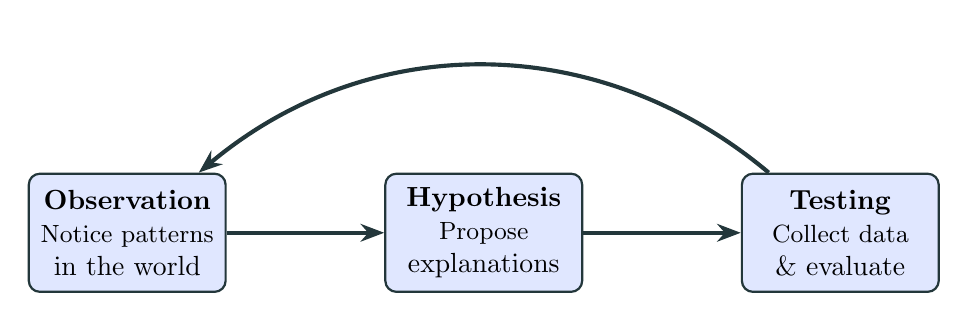
\begin{tikzpicture}[node distance=2cm, auto, thick]
    \node[rectangle, rounded corners, draw=myDarkTeal, fill=customlightblue, minimum width=2.5cm, minimum height=1.5cm, align=center] (obs) {\textbf{Observation}\\\small Notice patterns\\in the world};
    
    \node[rectangle, rounded corners, draw=myDarkTeal, fill=customlightblue, minimum width=2.5cm, minimum height=1.5cm, align=center, right=of obs] (hyp) {\textbf{Hypothesis}\\\small Propose\\explanations};
    
    \node[rectangle, rounded corners, draw=myDarkTeal, fill=customlightblue, minimum width=2.5cm, minimum height=1.5cm, align=center, right=of hyp] (test) {\textbf{Testing}\\\small Collect data\\\& evaluate};
    
    \draw[-{Stealth[length=3mm]}, line width=1.5pt, myDarkTeal] (obs) -- (hyp);
    \draw[-{Stealth[length=3mm]}, line width=1.5pt, myDarkTeal] (hyp) -- (test);
    \draw[-{Stealth[length=3mm]}, line width=1.5pt, myDarkTeal] (test) to[bend right=40] (obs);
\end{tikzpicture}
\end{center}

\vspace{0.5cm}
\begin{block}{}
\centering
\textbf{Science is iterative, not linear}\\
Each cycle refines our understanding and generates new questions
\end{block}
\end{frame}

% Slide 3: Example of Scientific Cycle
{\usebackgroundtemplate{ \includegraphics[height=\paperwidth]{imgs/EMpylori_lighter.jpg}} 
	\begin{frame}{Example: Discovery of \textit{Helicobacter pylori}}
		\begin{block}{Observation (1980s)}
			Most stomach ulcers occur in similar patterns; some patients don't respond to stress-reduction treatments
		\end{block}

		\begin{block}{Hypothesis}
			Ulcers might be caused by bacterial infection, not just stress or spicy food
		\end{block}

		\begin{block}{Testing}
			Collected stomach tissue samples, cultured bacteria, tested antibiotics on patients
		\end{block}

		\begin{alertblock}{Result}
			\textit{H. pylori} confirmed as cause → paradigm shift in treatment → Nobel Prize 2005
		\end{alertblock}
		\end{frame}
	}

% Slide 4: Data as Evidence
\begin{frame}{The Role of Data as Evidence}
\begin{center}
Data serves as the \textbf{empirical bridge} between our ideas about the world and the world itself
\end{center}

\vspace{0.5cm}
\begin{columns}[T]
\begin{column}{0.48\textwidth}
\begin{block}{Without Data}
\begin{itemize}
\item Speculation and opinion
\item Anecdote and intuition
\item Unverified assumptions
\item Competing narratives
\end{itemize}
\end{block}
\end{column}

\begin{column}{0.48\textwidth}
\begin{exampleblock}{With Data}
\begin{itemize}
\item Evidence-based claims
\item Systematic observation
\item Testable predictions
\item Reproducible findings
\end{itemize}
\end{exampleblock}
\end{column}
\end{columns}

\vspace{0.5cm}
\begin{center}
\textit{``In God we trust. All others must bring data.''} \\
— W. Edwards Deming
\end{center}
\end{frame}

% Slide 5: Building Scientific Knowledge
\begin{frame}{Building and Refining Scientific Knowledge}
\framesubtitle{Science as Cumulative Process}

\begin{itemize}
\item \textbf{Incremental Progress} \\
Each study adds a piece to the puzzle, building on previous work

\vspace{0.3cm}
\item \textbf{Self-Correction} \\
Replication and peer review help identify and correct errors

\vspace{0.3cm}
\item \textbf{Increasing Precision} \\
Better methods and more data → more accurate understanding

\vspace{0.3cm}
\item \textbf{Paradigm Shifts} \\
Occasionally, accumulated evidence forces revolutionary rethinking
\end{itemize}
\end{frame}

% Slide 6: Descriptive vs Inferential
\begin{frame}{Descriptive vs. Inferential Science}
\begin{columns}[T]
\begin{column}{0.48\textwidth}
\begin{block}{Descriptive Science}
\textbf{Goal:} Characterize what is observed

\vspace{0.3cm}
\textbf{Questions:}
\begin{itemize}
\item What patterns exist?
\item How much/many?
\item What are the characteristics?
\end{itemize}

\vspace{0.3cm}
\textbf{Example:} Measuring the average height of students in this class
\end{block}
\end{column}

\begin{column}{0.50\textwidth}
\begin{block}{Inferential Science}
\textbf{Goal:} Generalize beyond observations

\vspace{0.3cm}
\textbf{Questions:}
\begin{itemize}
\item Does this apply broadly?
\item Is this effect real?
\item What can we predict?
\end{itemize}

\vspace{0.3cm}
\textbf{Example:} Using class data to estimate average height of all university students
\end{block}
\end{column}
\end{columns}

\vspace{0.5cm}
\begin{center}
\textbf{Most data analysis involves both:} describe your sample, then infer about the population
\end{center}
\end{frame}

% Slide 7: Example - Clinical Trial
\begin{frame}{Example: From Description to Inference}
\framesubtitle{Clinical Trial for Blood Pressure Medication}

\begin{block}{Descriptive Phase}
In our trial of 500 patients, the treatment group (n=250) showed an average reduction of 15 mmHg, while the control group (n=250) showed 3 mmHg reduction
\end{block}

\begin{center}
$\Downarrow$
\end{center}
\pause
\begin{alertblock}{Inferential Phase}
\textbf{Question:} Is this 12 mmHg difference likely to be real for all similar patients, or just a fluke in our sample?

\vspace{0.2cm}
\textbf{Statistical inference:} Calculate probability that difference this large could occur by chance (p-value), estimate range for true effect (confidence interval)
\end{alertblock}

\begin{exampleblock}{Conclusion}
If $p < 0.05$ and confidence interval doesn't include zero → we infer the drug likely works for broader population beyond just our 500 patients
\end{exampleblock}
\end{frame}


% Slide 9: Statistics vs Causation
\begin{frame}{Statistics Alone Cannot Determine Causes}
\framesubtitle{The Limits of Correlation}

\begin{alertblock}{Key Principle}
Correlation does not imply causation
\end{alertblock}

\vspace{0.3cm}

\begin{exampleblock}{Classic Example: Ice Cream and Drowning}
\textbf{Observation:} Ice cream sales and drowning deaths are strongly correlated

\vspace{0.2cm}
\textbf{Statistical finding:} High correlation ($r \approx 0.9$)
\pause
\vspace{0.2cm}
\textbf{Wrong conclusion:} Ice cream causes drowning (or vice versa)
\pause
\vspace{0.2cm}
\textbf{Actual mechanism:} Both increase during summer; temperature is the \alert{confounding variable}
\end{exampleblock}

\vspace{0.3cm}

\textbf{Why statistics alone isn't enough:}
\begin{itemize}
\item Can identify associations but not causal direction
\item Cannot distinguish direct from indirect effects
\item Cannot reveal confounding variables without assumptions
\end{itemize}
\end{frame}

% Slide 10: Three Types of Relationships
\begin{frame}{Understanding Different Types of Relationships}

\begin{columns}[T]
\begin{column}{0.32\textwidth}
\begin{block}{Direct Causation}
\centering
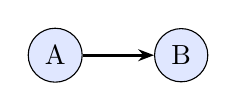
\begin{tikzpicture}[scale=0.8]
    \node[circle, draw, fill=customlightblue] (A) at (0,0) {A};
    \node[circle, draw, fill=customlightblue] (B) at (2,0) {B};
    \draw[-{Stealth[length=2mm]}, line width=1pt] (A) -- (B);
\end{tikzpicture}

\vspace{0.2cm}
A causes B %\small Smoking → Lung Cancer
\end{block}
\end{column}


\begin{column}{0.32\textwidth}
\begin{block}{Reverse Causation}
\centering
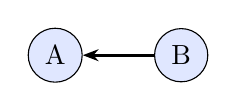
\begin{tikzpicture}[scale=0.8]
    \node[circle, draw, fill=customlightblue] (A) at (0,0) {A};
    \node[circle, draw, fill=customlightblue] (B) at (2,0) {B};
    \draw[-{Stealth[length=2mm]}, line width=1pt] (B) -- (A);
\end{tikzpicture}

\vspace{0.2cm}
B causes A %\small Disease → Hospital Visit (not vice versa)
\end{block}
\end{column}
\end{columns}


\pause
\begin{center}
\alert{\bf Basic Confounds}
\end{center}
\begin{columns}[T]

% the fork
\begin{column}{0.32\textwidth}
\begin{block}{The fork}
\centering
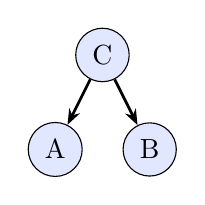
\begin{tikzpicture}[scale=0.8]
    \node[circle, draw, fill=customlightblue] (C) at (0,1.5) {C};
    \node[circle, draw, fill=customlightblue] (A) at (-0.75,0) {A};
    \node[circle, draw, fill=customlightblue] (B) at (0.75,0) {B};
    \draw[-{Stealth[length=2mm]}, line width=1pt] (C) -- (A);
    \draw[-{Stealth[length=2mm]}, line width=1pt] (C) -- (B);
\end{tikzpicture}

\vspace{0.2cm}
C is common cause to A and B%\small Temperature → Ice Cream \& Drowning
\end{block}
\end{column}

	
% the pipe
\begin{column}{0.32\textwidth}
\begin{block}{The pipe}
\centering
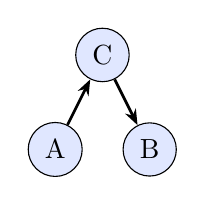
\begin{tikzpicture}[scale=0.8]
    \node[circle, draw, fill=customlightblue] (C) at (0,1.5) {C};
    \node[circle, draw, fill=customlightblue] (A) at (-0.75,0) {A};
    \node[circle, draw, fill=customlightblue] (B) at (0.75,0) {B};
    \draw[-{Stealth[length=2mm]}, line width=1pt] (A) -- (C);
    \draw[-{Stealth[length=2mm]}, line width=1pt] (C) -- (B);
\end{tikzpicture}

\vspace{0.2cm}
C is a \textit{mediator} of the effect of A on B %\small Temperature → Ice Cream \& Drowning
\end{block}
\end{column}


% the collider
\begin{column}{0.32\textwidth}
\begin{block}{The collider}
\centering
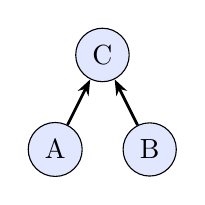
\begin{tikzpicture}[scale=0.8]
    \node[circle, draw, fill=customlightblue] (C) at (0,1.5) {C};
    \node[circle, draw, fill=customlightblue] (A) at (-0.75,0) {A};
    \node[circle, draw, fill=customlightblue] (B) at (0.75,0) {B};
    \draw[-{Stealth[length=2mm]}, line width=1pt] (A) -- (C);
    \draw[-{Stealth[length=2mm]}, line width=1pt] (B) -- (C);
\end{tikzpicture}

\vspace{0.2cm}
A and B cause C%\small Temperature → Ice Cream \& Drowning
\end{block}
\end{column}

\end{columns}


\vspace{-0.2cm}
\begin{center}
\alert{Statistics identifies associations; models explain mechanisms}
\end{center}
\end{frame}

% Slide 11: Mechanistic Models
\begin{frame}{The Power of Mechanistic Models}
\framesubtitle{Understanding How Things Work}

\begin{block}{What are Mechanistic Models?}
Models that explicitly represent the \textbf{underlying processes} and \textbf{causal mechanisms} that generate observed patterns
\end{block}

\vspace{0.3cm}

\begin{columns}[T]
\begin{column}{0.48\textwidth}
\textbf{Statistical Models:}
\begin{itemize}
\item Describe patterns
\item Make predictions
\item Quantify uncertainty
\item "What" happens
\end{itemize}
\end{column}

\begin{column}{0.48\textwidth}
\textbf{Mechanistic Models:}
\begin{itemize}
\item Explain processes
\item Test mechanisms
\item Guide interventions
\item "How" and "why" it happens
\end{itemize}
\end{column}
\end{columns}

\vspace{0.4cm}

\begin{exampleblock}{Example: Epidemic Spread}
\textbf{Statistical:} Cases increasing exponentially with rate $r$

\textbf{Mechanistic:} SIR model—susceptible individuals become infected through contact, then recover with immunity. This explains \emph{why} the pattern changes over time.
\end{exampleblock}
\end{frame}

% Slide 12: Benefits of Mechanistic Models
\begin{frame}{Why Mechanistic Models Matter}

\begin{itemize}[<+->] 
\item \textbf{Intervention Design} \\
Understanding mechanisms tells us \emph{where} to intervene \\
\textit{Example:} Knowing malaria transmission requires mosquitoes → target mosquito populations

\vspace{0.3cm}
\item \textbf{Extrapolation} \\
Mechanistic models generalize better to new situations \\
\textit{Example:} Physics equations work on Earth and Mars; purely statistical models trained on Earth data might not

\vspace{0.3cm}
\item \textbf{Counterfactual Reasoning} \\
Can answer "what if" questions about things we haven't observed \\
\textit{Example:} What would happen if we removed this gene? Changed this policy?

\vspace{0.3cm}
\item \textbf{Insight and Understanding} \\
Reveals the fundamental principles governing a system \\
\textit{Example:} Newton's laws explain both falling apples and planetary orbits
\end{itemize}
\end{frame}

% Slide 13: Integration
\begin{frame}{Integrating Statistics and Mechanism}
\framesubtitle{The Best of Both Worlds}

\begin{center}
\textbf{Modern data analysis combines both approaches}
\end{center}

\vspace{0.3cm}

\begin{block}{The Workflow}
\begin{enumerate}
\item Use \textbf{statistical methods} to identify patterns and associations
\item Develop \textbf{mechanistic hypotheses} to explain those patterns
\item Use \textbf{statistics} to test mechanistic predictions
\item Refine the mechanism based on statistical evidence
\item Iterate!
\end{enumerate}
\end{block}

\vspace{0.3cm}

\begin{exampleblock}{Example: Drug Development}
\begin{itemize}
\item Statistics: Drug A correlates with improved outcomes
\item Mechanism: Drug A inhibits enzyme X, which blocks pathway Y
\item Prediction: Other enzyme X inhibitors should also work
\item Statistical test: Clinical trials confirm mechanism-based prediction
\end{itemize}
\end{exampleblock}
\end{frame}

% Slide 14: Key Takeaways
\begin{frame}{Key Takeaways}
\begin{enumerate}
\item Science is a \textbf{cyclical process} of observation, hypothesis, and testing—not a one-way street

\vspace{0.3cm}
\item Data provides the \textbf{empirical evidence} that grounds our scientific claims in reality

\vspace{0.3cm}
\item Scientific knowledge is \textbf{cumulative and self-correcting}, building over time through many studies

\vspace{0.3cm}
\item We use \textbf{descriptive} methods to characterize what we observe and \textbf{inferential} methods to generalize beyond our data

\vspace{0.3cm}
\item \alert{Statistics alone cannot determine causation}—we need models that represent mechanisms

\vspace{0.3cm}
\item \textbf{Mechanistic models} explain how and why phenomena occur, enabling better predictions and interventions
\end{enumerate}

\vspace{0.5cm}
\begin{center}
\colorbox{myOrange}{\textcolor{white}{\parbox{0.9\textwidth}{\centering\textbf{Data analysis is the engine that powers this entire scientific process}}}}
\end{center}
\end{frame}

\section{The bridge between raw observations and scientific understanding}
% Slide 1: Title
%\begin{frame}
%\titlepage
%\begin{center}
%\textit{The bridge between raw observations and scientific understanding}
%\end{center}
%\end{frame}

% Slide 2: Defining Data Analysis
\begin{frame}{What is Data Analysis?}

\begin{block}{Definition}
Data analysis is the process of \textbf{transforming raw data} into \textbf{meaningful insights} through systematic examination, cleaning, modeling, and interpretation
\end{block}

\vspace{0.5cm}

\begin{center}
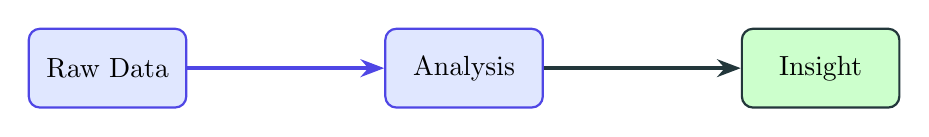
\begin{tikzpicture}[node distance=2.5cm, auto, thick]
    \node[rectangle, rounded corners, draw=customblue, fill=customlightblue, minimum width=2cm, minimum height=1cm] (raw) {Raw Data};
    
    \node[rectangle, rounded corners, draw=customblue, fill=customlightblue, minimum width=2cm, minimum height=1cm, right=of raw] (analysis) {Analysis};
    
    \node[rectangle, rounded corners, draw=myDarkTeal, fill=green!20, minimum width=2cm, minimum height=1cm, right=of analysis] (insight) {Insight};
    
    \draw[-{Stealth[length=3mm]}, line width=1.5pt, customblue] (raw) -- (analysis);
    \draw[-{Stealth[length=3mm]}, line width=1.5pt, myDarkTeal] (analysis) -- (insight);
\end{tikzpicture}
\end{center}

\vspace{0.5cm}

Data analysis is:
\begin{itemize}
\item The \alert{bridge} between observation and understanding
\item Both a \textbf{technical skill} and an \textbf{art of reasoning}
\item Essential to making \textbf{evidence-based decisions}
\end{itemize}
\end{frame}

% Slide 3: Exploratory vs Confirmatory
\begin{frame}{Two Modes of Data Analysis}

\begin{columns}[T]
\begin{column}{0.48\textwidth}
\begin{block}{Exploratory Analysis}
\textbf{Goal:} Discover patterns and generate hypotheses

\vspace{0.3cm}
\textbf{Approach:}
\begin{itemize}
\item Open-ended investigation
\item Visualization-heavy
\item Flexible methods
\item Pattern recognition
\end{itemize}

\vspace{0.3cm}
\textbf{Mindset:} \\
\textit{"What's in this data?"}

\vspace{0.2cm}
\small \textbf{Example:} Plotting gene expression data to identify clusters of co-regulated genes
\end{block}
\end{column}

\begin{column}{0.48\textwidth}
\begin{block}{Confirmatory Analysis}
\textbf{Goal:} Test specific hypotheses rigorously

\vspace{0.3cm}
\textbf{Approach:}
\begin{itemize}
\item Pre-specified questions
\item Formal statistical tests
\item Control for error rates
\item Hypothesis testing
\end{itemize}

\vspace{0.3cm}
\textbf{Mindset:} \\
\textit{"Is this effect real?"}

\vspace{0.2cm}
\small \textbf{Example:} Testing whether Gene A expression differs significantly between treatment and control groups
\end{block}
\end{column}
\end{columns}

\vspace{0.4cm}
\begin{center}
\alert{Both are essential!} Exploration discovers, confirmation validates
\end{center}
\end{frame}

% Slide 4: The Dangers of Conflating
\begin{frame}{Don't Confuse Exploration with Confirmation}

\begin{alertblock}{The Problem}
Using the same data to both generate and test hypotheses leads to \textbf{false discoveries} and \textbf{inflated confidence}
\end{alertblock}

\vspace{0.3cm}

\begin{exampleblock}{Example: The Garden of Forking Paths}
\begin{enumerate}
\item Explore data, notice that variable X correlates with outcome Y
\item Test this correlation on the same data → $p < 0.05$!
\item Conclude X causes Y with high confidence
\item \alert{Problem:} You found the correlation by exploring many variables; the test is invalid
\end{enumerate}
\end{exampleblock}

\vspace{0.3cm}

\textbf{Best Practices:}
\begin{itemize}
\item Use separate datasets for exploration and confirmation
\item Pre-register hypotheses before confirmatory analysis
\item Be transparent about which analyses were planned vs. exploratory
\item Adjust for multiple comparisons when testing many hypotheses
\end{itemize}
\end{frame}

% Slide 5: Data Analysis as Technical Skill
\begin{frame}{Data Analysis as Technical Skill}

\textbf{The Technical Toolkit:}

\begin{columns}[T]
\begin{column}{0.48\textwidth}
\begin{block}{Statistical Methods}
\begin{itemize}
\item Descriptive statistics
\item Probability distributions
\item Hypothesis testing
\item Regression modeling
\item Machine learning
\item Bayesian inference
\end{itemize}
\end{block}
\end{column}

\begin{column}{0.48\textwidth}
\begin{block}{Practical Skills}
\begin{itemize}
\item Data cleaning \& wrangling
\item Programming (R, Python)
\item Visualization
\item Database queries
\item Reproducible workflows
\item Version control
\end{itemize}
\end{block}
\end{column}
\end{columns}

\vspace{0.5cm}

\begin{center}
These are \textbf{learnable skills} that improve with practice \\
\small (We'll cover many of these throughout the course)
\end{center}
\end{frame}

% Slide 6: Data Analysis as Art
\begin{frame}{Data Analysis as Art of Reasoning}

\textbf{Beyond the formulas, data analysis requires:}

\vspace{0.3cm}

\begin{itemize}
\item \textbf{Judgment} — Which method is appropriate for this question?

\vspace{0.2cm}
\item \textbf{Creativity} — How can I visualize this pattern effectively?

\vspace{0.2cm}
\item \textbf{Critical thinking} — Does this result make sense? What could go wrong?

\vspace{0.2cm}
\item \textbf{Domain knowledge} — What do I know about the subject matter that informs analysis?

\vspace{0.2cm}
\item \textbf{Communication} — How do I explain these findings clearly to others?

\vspace{0.2cm}
\item \textbf{Skepticism} — Am I seeing a real pattern or being fooled by randomness?
\end{itemize}

\vspace{0.4cm}

\begin{alertblock}{}
\centering
Good data analysis combines \textbf{technical proficiency} with \textbf{thoughtful reasoning}
\end{alertblock}
\end{frame}

% Slide 7: Example of Judgment
\begin{frame}{Example: When Technical Skills Meet Reasoning}
\framesubtitle{Choosing the Right Average}

\begin{exampleblock}{Scenario: Income Data}
You're analyzing household income in a neighborhood: \\
\$35k, \$42k, \$38k, \$45k, \$40k, \$2.5M, \$37k, \$41k

\vspace{0.3cm}
\textbf{Technical calculation:}
\begin{itemize}
\item Mean = \$348,625
\item Median = \$40,500
\end{itemize}
\end{exampleblock}

\vspace{0.3cm}

\textbf{Which is "correct"?}

\begin{itemize}
\item \alert{Technical skill:} Both are calculated correctly
\item \alert{Judgment:} Median better represents typical household (mean distorted by outlier)
\item \alert{Critical thinking:} Why is there one very high value? Data error or billionaire resident?
\item \alert{Communication:} Report both, explain why median is more meaningful here
\end{itemize}
\end{frame}

% Slide 8: The Role of Uncertainty
\begin{frame}{Data Analysis and Uncertainty}

\begin{block}{Core Principle}
All data analysis involves \textbf{uncertainty}—our goal is to \alert{quantify and communicate} it honestly
\end{block}

\vspace{0.3cm}

\textbf{Sources of Uncertainty:}

\begin{itemize}
\item \textbf{Sampling variability} — We observe a sample, not the entire population

\vspace{0.2cm}
\item \textbf{Measurement error} — Our instruments and methods aren't perfect

\vspace{0.2cm}
\item \textbf{Model uncertainty} — Our models are simplifications of reality

\vspace{0.2cm}
\item \textbf{Unknown confounders} — Variables we didn't measure might matter
\end{itemize}

\vspace{0.4cm}

\begin{center}
\textit{``The only certainty is that nothing is certain''} — Pliny the Elder

\vspace{0.2cm}
Good analysts embrace uncertainty rather than hide from it
\end{center}
\end{frame}

% Slide 9: Quantifying Uncertainty
\begin{frame}{Tools for Quantifying Uncertainty}

\textbf{How we express uncertainty in data analysis:}

\vspace{0.3cm}

\begin{block}{Confidence Intervals}
Range of plausible values for a parameter \\
\textit{Example:} "Average height is 170cm (95\% CI: 168-172cm)"
\end{block}

\begin{block}{P-values}
Probability of observing data this extreme if null hypothesis is true \\
\textit{Example:} "$p = 0.03$ means 3\% chance of this result by chance alone"
\end{block}

\begin{block}{Prediction Intervals}
Range where future observations are likely to fall \\
\textit{Example:} "Next patient's blood pressure: 120 mmHg (90\% PI: 100-140)"
\end{block}

\vspace{0.3cm}

\begin{center}
\small These tools help us distinguish \alert{signal from noise}
\end{center}
\end{frame}

% Slide 10: Data Analysis in Context
\begin{frame}{Data Analysis Never Happens in Vacuum}

\begin{center}
\textbf{Every analysis serves a purpose}
\end{center}

\vspace{0.3cm}

\textbf{Consider the context:}

\begin{itemize}
\item \textbf{Who} will use these results?
\item \textbf{What} decision needs to be made?
\item \textbf{Why} is this question important?
\item \textbf{When} do results need to be ready?
\item \textbf{How} will findings be communicated?
\end{itemize}

\vspace{0.4cm}

\begin{exampleblock}{Example: Clinical Trial Analysis}
\begin{itemize}
\item \textbf{Who:} Doctors, patients, regulators
\item \textbf{What:} Approve drug or not?
\item \textbf{Why:} Patient lives at stake
\item \textbf{Result:} Need higher standards of evidence, clearer communication of risks
\end{itemize}
\end{exampleblock}
\end{frame}

% Slide 11: Common Pitfalls
\begin{frame}{Common Pitfalls in Data Analysis}

\begin{enumerate}
\item \textbf{P-hacking} \\
\small Trying many analyses until finding $p < 0.05$

\vspace{0.2cm}
\item \textbf{HARKing} (Hypothesizing After Results are Known) \\
\small Pretending you predicted what you actually discovered

\vspace{0.2cm}
\item \textbf{Cherry-picking} \\
\small Reporting only results that support your hypothesis

\vspace{0.2cm}
\item \textbf{Confusing correlation with causation} \\
\small Assuming association implies causal relationship

\vspace{0.2cm}
\item \textbf{Ignoring assumptions} \\
\small Applying methods without checking if assumptions are met

\vspace{0.2cm}
\item \textbf{Overfitting} \\
\small Creating models that fit your data perfectly but predict poorly

\vspace{0.2cm}
\item \textbf{Survivorship bias} \\
\small Analyzing only successful cases while ignoring failures
\end{enumerate}
\end{frame}

% Slide 12: Best Practices
\begin{frame}{Best Practices for Rigorous Data Analysis}

\begin{block}{Before Analysis}
\begin{itemize}
\item Clearly define your research question
\item Pre-register your analysis plan (when possible)
\item Understand your data's origin and limitations
\end{itemize}
\end{block}

\begin{block}{During Analysis}
\begin{itemize}
\item Document every step (reproducibility!)
\item Check assumptions of your methods
\item Visualize data before modeling
\item Consider alternative explanations
\end{itemize}
\end{block}

\begin{block}{After Analysis}
\begin{itemize}
\item Report all analyses performed, not just significant ones
\item Be transparent about limitations
\item Distinguish between exploratory and confirmatory findings
\item Make data and code available (when appropriate)
\end{itemize}
\end{block}
\end{frame}

% Slide 13: The Data Analysis Workflow Preview
\begin{frame}{Preview: The Data Analysis Pipeline}
\framesubtitle{We'll explore this in detail throughout the course}

\begin{center}
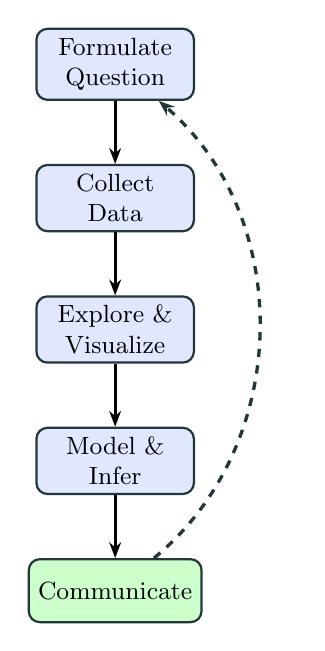
\begin{tikzpicture}[node distance=0.8cm, auto, thick, every node/.style={font=\small}]
    \node[rectangle, rounded corners, draw=myDarkTeal, fill=customlightblue, minimum width=2cm, minimum height=0.8cm, align=center] (question) {Formulate\\Question};
    
    \node[rectangle, rounded corners, draw=myDarkTeal, fill=customlightblue, minimum width=2cm, minimum height=0.8cm, align=center, below=of question] (collect) {Collect\\Data};
    
    \node[rectangle, rounded corners, draw=myDarkTeal, fill=customlightblue, minimum width=2cm, minimum height=0.8cm, align=center, below=of collect] (explore) {Explore \&\\Visualize};
    
    \node[rectangle, rounded corners, draw=myDarkTeal, fill=customlightblue, minimum width=2cm, minimum height=0.8cm, align=center, below=of explore] (model) {Model \&\\Infer};
    
    \node[rectangle, rounded corners, draw=myDarkTeal, fill=green!20, minimum width=2cm, minimum height=0.8cm, align=center, below=of model] (communicate) {Communicate};
    
    \draw[-{Stealth[length=2mm]}, line width=1.2pt] (question) -- (collect);
    \draw[-{Stealth[length=2mm]}, line width=1.2pt] (collect) -- (explore);
    \draw[-{Stealth[length=2mm]}, line width=1.2pt] (explore) -- (model);
    \draw[-{Stealth[length=2mm]}, line width=1.2pt] (model) -- (communicate);

    \draw[-{Stealth[length=2mm]}, line width=1.2pt, dashed, myDarkTeal] (communicate) to[bend right=50] (question);
\end{tikzpicture}
\end{center}

\vspace{0.2cm}
Each stage involves both \alert{technical skills} and \alert{critical thinking}
\end{frame}

% Slide 14: Key Takeaways
\begin{frame}{Key Takeaways}

\begin{enumerate}
\item Data analysis is the \textbf{bridge} between raw observations and scientific understanding

\vspace{0.3cm}
\item \textbf{Exploratory} analysis discovers patterns; \textbf{confirmatory} analysis tests hypotheses—don't confuse them!

\vspace{0.3cm}
\item Data analysis requires both \textbf{technical proficiency} and \textbf{thoughtful reasoning}

\vspace{0.3cm}
\item All analysis involves \alert{uncertainty}—our job is to quantify and communicate it honestly

\vspace{0.3cm}
\item Beware common pitfalls: p-hacking, cherry-picking, confusing correlation with causation

\vspace{0.3cm}
\item Good analysis is \textbf{transparent}, \textbf{reproducible}, and considers the broader context
\end{enumerate}

\vspace{0.5cm}
\begin{center}
\colorbox{myOrange}{\textcolor{white}{\parbox{0.9\textwidth}{\centering\textbf{Data analysis is both a science and an art\\—master both!}}}}
\end{center}
\end{frame}

\section{The deep questions underlying statistical inference}

% Slide 1: Title
%\begin{frame}
%\titlepage
%\begin{center}
%\textit{The deep questions underlying statistical inference}
%\end{center}
%\end{frame}


% Slide 2: Why Philosophy Matters
\begin{frame}{Why Philosophy Matters for Data Analysis}

\begin{alertblock}{The Core Question}
How do we gain reliable knowledge from limited, uncertain observations?
\end{alertblock}

\vspace{0.3cm}

\textbf{Philosophical questions shape practical decisions:}

\begin{itemize}
\item How much evidence is enough to conclude something is real?
\item What does "probability" actually mean?
\item Can we ever prove causation from observational data?
\item How should prior knowledge influence our conclusions?
\item What makes one explanation better than another?
\end{itemize}

\vspace{0.4cm}

\begin{center}
These aren't just abstract questions—they affect how we \alert{design studies}, \alert{analyze data}, and \alert{interpret results} in biology every day
\end{center}
\end{frame}

% Slide 3: Section A - Epistemology
\begin{frame}{A. Epistemology: How Do We Know What We Know?}
\framesubtitle{The Study of Knowledge and Justification}

\begin{block}{Epistemology}
The branch of philosophy concerned with the nature, sources, and limits of knowledge
\end{block}

\vspace{0.3cm}

\textbf{Key Questions for Scientists:}

\begin{enumerate}
\item What counts as evidence?
\item How do we justify believing our conclusions?
\item What are the limits of what we can know from data?
\item How certain do we need to be before acting?
\end{enumerate}

\vspace{0.4cm}

\begin{exampleblock}{In Biology}
When we sequence a genome, how do we know the sequence is correct? \\
When we observe a correlation, how do we know it's real and not chance?
\end{exampleblock}
\end{frame}

% Slide 4: The Problem of Induction
\begin{frame}{The Problem of Induction}
\framesubtitle{Moving from Specific to General}

\begin{block}{Inductive Reasoning}
Drawing general conclusions from specific observations
\end{block}

\vspace{0.3cm}

\begin{columns}[T]
\begin{column}{0.48\textwidth}
\textbf{The Logic:}
\begin{enumerate}
\item Observed: Swan 1 is white
\item Observed: Swan 2 is white
\item Observed: Swan 3 is white
\item ... (1000 swans)
\item \alert{Conclude:} All swans are white
\end{enumerate}
\end{column}

\begin{column}{0.48\textwidth}
\textbf{The Problem:}
\begin{itemize}
\item We can't observe \emph{all} swans
\item Next swan could be black
\item No matter how many white swans we see, we can't be \emph{certain}
\item Yet science relies on this!
\end{itemize}
\end{column}
\end{columns}

\vspace{0.4cm}

\begin{center}
\small (And indeed, black swans exist in Australia—discovered 1697)
\end{center}
\end{frame}

% Slide 5: Induction in Biology
\begin{frame}{The Problem of Induction in Biology}

\begin{exampleblock}{Example: Drug Testing}
\textbf{Observation:} New drug reduces tumor size in 100 mice

\vspace{0.2cm}
\textbf{Inductive inference:} Drug will reduce tumors in humans

\vspace{0.2cm}
\textbf{The problem:}
\begin{itemize}
\item We only tested 100 mice, not all mice
\item We tested mice, not humans
\item We tested under specific conditions
\item Future trials might fail
\end{itemize}
\end{exampleblock}

\vspace{0.3cm}

\textbf{How do we proceed despite uncertainty?}

\begin{itemize}
\item Use \alert{statistical inference} to quantify uncertainty
\item Require \alert{replication} across studies
\item Test in \alert{multiple model systems} before humans
\item Accept that science gives us \alert{provisional knowledge}, not certainty
\end{itemize}
\end{frame}

% Slide 6: Uncertainty is Inherent
\begin{frame}{Uncertainty is Inherent in Empirical Knowledge}

\begin{center}
\Large \alert{There is no escape from uncertainty in science}
\end{center}

\vspace{0.3cm}

\textbf{Why statistical thinking is essential:}

\begin{itemize}
\item We can never observe everything (all cells, all organisms, all conditions)
\item Biological systems are inherently variable
\item Measurements contain error
\item Chance events occur
\end{itemize}

\vspace{0.4cm}

\begin{block}{The Solution}
Statistics provides tools to:
\begin{itemize}
\item \textbf{Quantify} how uncertain we should be
\item \textbf{Distinguish} real patterns from random noise
\item \textbf{Make decisions} with explicit error rates
\end{itemize}
\end{block}

\vspace{0.1cm}

\begin{center}
\textit{Statistics is the grammar of science in the face of uncertainty}
\end{center}
\end{frame}

% Slide 7: Models and Reality
\begin{frame}{B. Models and Reality}
\framesubtitle{The Map is Not the Territory}

\begin{center}
\large \textit{``All models are wrong, \\but some are useful''}

\vspace{0.3cm}
\normalsize — George E.P. Box
\end{center}

\vspace{0.5cm}

\begin{block}{What This Means}
\begin{itemize}
\item Every model (statistical or mechanistic) is a \alert{simplification} of reality
\item No model captures every detail—nor should it
\item The question is not "Is this model true?" but "Is it useful?"
\item Good models capture essential features while ignoring irrelevant complexity
\end{itemize}
\end{block}

\vspace{0.3cm}

\begin{center}
Like a map: it's not the actual terrain, but it helps you navigate
\end{center}
\end{frame}

% Slide 8: Models in Biology
\begin{frame}{Statistical Models in Biology}

\begin{exampleblock}{Example: Linear Regression for Gene Expression}
\textbf{Model:} Expression = $\beta_0$ + $\beta_1 \times$ Temperature + error
\end{exampleblock}


\vspace{0.2cm}


\begin{columns}[T]
	\begin{column}{0.48\textwidth}
\textbf{What the model assumes:}
\begin{itemize}
\item Linear relationship
\item Constant variance
\item Independent observations
\item Normally distributed errors
\end{itemize}
  \end{column}
%\vspace{0.2cm}
	\begin{column}{0.48\textwidth}
\textbf{Reality:}
\begin{itemize}
\item Relationship might be curved at extremes
\item Variance might change with temperature
\item Gene networks create dependencies
\item Distributions might be skewed
\end{itemize}
  \end{column}
\end{columns}

\vspace{0.3cm}

\textbf{Is the model wrong?} Yes. \textbf{Is it useful?} Often! \\
It captures the main trend and lets us make predictions

\end{frame}

% Slide 9: Choosing Models
\begin{frame}{Choosing Between Models}

\textbf{How do we decide which model to use?}

\vspace{0.3cm}

\begin{enumerate}
\item \textbf{Purpose} — What question are we trying to answer?

\vspace{0.2cm}
\item \textbf{Assumptions} — Which model's assumptions are most reasonable?

\vspace{0.2cm}
\item \textbf{Fit vs. Simplicity} — Balance between accuracy and parsimony

\vspace{0.2cm}
\item \textbf{Interpretability} — Can we understand what the model tells us?

\vspace{0.2cm}
\item \textbf{Generalizability} — Will it work on new data?
\end{enumerate}

\vspace{0.4cm}

\begin{alertblock}{Occam's Razor}
\textit{``Entities should not be multiplied beyond necessity''} \\
When two models explain the data equally well, prefer the simpler one
\end{alertblock}
\end{frame}

% Slide 10: Example - Complexity Trade-off
\begin{frame}{Example: The Complexity Trade-off}
\framesubtitle{Modeling Plant Growth vs. Nutrients}

\begin{columns}[T]
\begin{column}{0.48\textwidth}
\textbf{Simple Model:} \\
Growth = $a$ + $b \times$ Nitrogen

\vspace{0.3cm}
\textbf{Pros:}
\begin{itemize}
\item Easy to interpret
\item Few parameters
\item Stable predictions
\end{itemize}

\vspace{0.2cm}
\textbf{Cons:}
\begin{itemize}
\item Misses saturation effect
\item Ignores other nutrients
\end{itemize}
\end{column}

\begin{column}{0.48\textwidth}
\textbf{Complex Model:} \\
Growth = $f$(N, P, K, pH, temp, \\
light, water, ...) with interactions

\vspace{0.1cm}
\textbf{Pros:}
\begin{itemize}
\item More realistic
\item Better fit to training data
\item Captures interactions
\end{itemize}

\vspace{0.2cm}
\textbf{Cons:}
\begin{itemize}
\item Hard to interpret
\item Many parameters
\item Might \alert{overfit}
\end{itemize}
\end{column}
\end{columns}

\vspace{0.4cm}

\begin{center}
\textbf{The art:} Finding the sweet spot between simplicity and realism
\end{center}
\end{frame}

% Slide 11: Objectivity and Subjectivity
\begin{frame}{C. Objectivity and Subjectivity in Analysis}

\begin{alertblock}{The Paradox}
Science aims for \textbf{objectivity}, but data analysis involves countless \textbf{subjective decisions}
\end{alertblock}

\vspace{0.3cm}

\textbf{Subjective choices analysts make:}

\begin{itemize}
\item Which variables to measure
\item How to define/categorize variables
\item Which data points to exclude (outliers?)
\item Which statistical test to use
\item How to transform data
\item Significance threshold ($\alpha = 0.05$?)
\item How to visualize results
\end{itemize}

\vspace{0.3cm}

\begin{center}
These are called \alert{``researcher degrees of freedom''}
\end{center}
\end{frame}

% Slide 12: Example - Researcher Degrees of Freedom
\begin{frame}{Example: Analyzing Cell Morphology}

\begin{exampleblock}{Scenario: Do cells change shape in response to drug?}

\textbf{Choice 1:} How to measure shape?
\begin{itemize}
\item Area? Perimeter? Aspect ratio? Circularity? All of them?
\end{itemize}

\textbf{Choice 2:} Which cells to include?
\begin{itemize}
\item Only complete cells? What about cells touching image border?
\item How to handle dividing cells?
\end{itemize}

\textbf{Choice 3:} How to handle outliers?
\begin{itemize}
\item Exclude cells $>$ 3 SD from mean? Or keep all?
\end{itemize}

\textbf{Choice 4:} Which statistical test?
\begin{itemize}
\item t-test? Wilcoxon test? Linear model with covariates?
\end{itemize}
\end{exampleblock}

\vspace{0.2cm}

Each choice is defensible—but different choices can lead to different conclusions!
\end{frame}

% Slide 13: The Replication Crisis
\begin{frame}{The Replication Crisis in Science}

\begin{block}{The Problem}
Many published findings fail to replicate when other labs try to reproduce them
\end{block}

\vspace{0.3cm}

\textbf{Contributing factors:}

\begin{itemize}
\item \textbf{P-hacking:} Trying many analyses until finding $p < 0.05$
\item \textbf{HARKing:} Hypothesizing After Results are Known
\item \textbf{Publication bias:} Journals prefer positive results
\item \textbf{Flexibility in analysis:} Using researcher degrees of freedom to get desired result
\item \textbf{Low statistical power:} Small samples lead to unreliable estimates
\end{itemize}

\vspace{0.3cm}

\begin{exampleblock}{Example from Psychology}
Study found that listening to "When I'm Sixty-Four" made people younger \\
\small (Result from p-hacking and selective reporting—obviously false)
\end{exampleblock}
\end{frame}

% Slide 14: Solutions - Pre-registration
\begin{frame}{Solution 1: Pre-registration and Transparency}

\begin{block}{Pre-registration}
Publicly specify your hypotheses, methods, and analysis plan \alert{before} collecting/analyzing data
\end{block}

\vspace{0.3cm}

\textbf{What to pre-register:}
\begin{itemize}
\item Research questions and hypotheses
\item Sample size and stopping rules
\item Which variables will be analyzed
\item Primary vs. secondary outcomes
\item Statistical tests and significance thresholds
\item Criteria for excluding data
\end{itemize}

\vspace{0.3cm}

\textbf{Benefits:}
\begin{itemize}
\item Prevents p-hacking and HARKing
\item Distinguishes confirmatory from exploratory analyses
\item Increases trust in results
\end{itemize}

\vspace{0.2cm}

\begin{center}
\small Platforms: OSF (osf.io), AsPredicted, ClinicalTrials.gov
\end{center}
\end{frame}

% Slide 15: Solutions - Open Science
\begin{frame}{Solution 2: Open Science Practices}

\textbf{Make research transparent and reproducible:}

\vspace{0.3cm}

\begin{block}{Open Data}
Share raw data (when ethically possible) so others can verify analyses
\end{block}

\begin{block}{Open Code}
Share analysis scripts so methods are completely transparent
\end{block}

\begin{block}{Open Materials}
Describe methods in enough detail for others to replicate
\end{block}

\vspace{0.3cm}

\begin{exampleblock}{Example in Biology}
Publishing sequencing data to GEO/SRA, sharing microscopy images, providing detailed protocols, making analysis code available on GitHub
\end{exampleblock}

\vspace{0.2cm}

\begin{center}
\alert{Transparency is the best antidote to bias}
\end{center}
\end{frame}

% Slide 16: Solutions - Reporting Standards
\begin{frame}{Solution 3: Better Reporting Standards}

\textbf{What journals and reviewers increasingly expect:}

\vspace{0.3cm}

\begin{itemize}
\item Report \alert{all} outcome measures, not just significant ones
\item Distinguish pre-planned from exploratory analyses
\item Report effect sizes with confidence intervals, not just p-values
\item Show data distributions, not just summary statistics
\item Acknowledge limitations honestly
\item Include negative results
\item Provide enough detail for replication
\end{itemize}

\vspace{0.4cm}

\begin{block}{Guidelines}
\begin{itemize}
\item CONSORT (clinical trials)
\item ARRIVE (animal research)
\item STROBE (observational studies)
\item PRISMA (systematic reviews)
\end{itemize}
\end{block}
\end{frame}

% Slide 17: Balancing Objectivity
\begin{frame}{Balancing Objectivity and Subjectivity}

\begin{center}
\textbf{We cannot eliminate subjectivity—but we can manage it}
\end{center}

\vspace{0.4cm}

\textbf{Best practices:}

\begin{enumerate}
\item \textbf{Acknowledge} that subjective choices exist

\vspace{0.2cm}
\item \textbf{Make choices explicit} through transparent reporting

\vspace{0.2cm}
\item \textbf{Pre-commit} to choices when possible (pre-registration)

\vspace{0.2cm}
\item \textbf{Test robustness} by trying alternative analysis approaches

\vspace{0.2cm}
\item \textbf{Seek independent replication} as ultimate test
\end{enumerate}

\vspace{0.4cm}

\begin{alertblock}{}
\centering
The goal is not to be perfectly objective (impossible) \\
but to be \alert{transparent and honest} about our choices
\end{alertblock}
\end{frame}

% Slide 18: Summary of Philosophical Tensions
\begin{frame}{Three Key Philosophical Tensions}

\begin{enumerate}
\item \textbf{Induction vs. Certainty} \\
\small We must generalize from limited data, accepting uncertainty is inevitable

\vspace{0.3cm}
\item \textbf{Simplicity vs. Realism} \\
\small Models must be simple enough to understand yet complex enough to be useful

\vspace{0.3cm}
\item \textbf{Objectivity vs. Subjectivity} \\
\small Science aims for objectivity but requires subjective judgment throughout
\end{enumerate}

\vspace{0.5cm}

\begin{center}
\alert{Good scientists navigate these tensions thoughtfully} \\
rather than pretending they don't exist
\end{center}
\end{frame}

% Slide 19: Key Takeaways
\begin{frame}{Key Takeaways}

\begin{enumerate}
\item \textbf{Induction problem:} We can never be certain, but statistics helps us quantify uncertainty

\vspace{0.3cm}
\item \textbf{Models are simplifications:} The question isn't "Is it true?" but "Is it useful?"

\vspace{0.3cm}
\item \textbf{All analysis involves subjective choices}—researcher degrees of freedom are real

\vspace{0.3cm}
\item \textbf{Flexibility in analysis} can lead to false discoveries (p-hacking, HARKing)

\vspace{0.3cm}
\item \textbf{Solutions:} Pre-registration, transparency, open science, better reporting

\vspace{0.3cm}
\item \textbf{Accept uncertainty and subjectivity}, but manage them through rigor and honesty
\end{enumerate}

\vspace{0.4cm}
\begin{center}
\colorbox{myOrange}{\textcolor{white}{\parbox{0.9\textwidth}{\centering\textbf{Understanding these foundations makes you a better, more thoughtful analyst}}}}
\end{center}
\end{frame}



\section{From question to insight}
% Slide 1: Title
%\begin{frame}
%\titlepage
%\begin{center}
%\textit{From question to insight: the journey of data analysis}
%\end{center}
%\end{frame}

% Slide 2: The Pipeline Overview

\begin{frame}{The Data Analysis Pipeline}
%\framesubtitle{We'll explore this in detail throughout the course}

\begin{center}
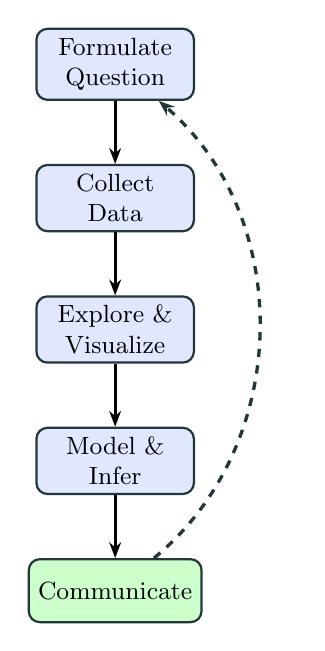
\begin{tikzpicture}[node distance=0.8cm, auto, thick, every node/.style={font=\small}]
    \node[rectangle, rounded corners, draw=myDarkTeal, fill=customlightblue, minimum width=2cm, minimum height=0.8cm, align=center] (question) {Formulate\\Question};
    
    \node[rectangle, rounded corners, draw=myDarkTeal, fill=customlightblue, minimum width=2cm, minimum height=0.8cm, align=center, below=of question] (collect) {Collect\\Data};
    
    \node[rectangle, rounded corners, draw=myDarkTeal, fill=customlightblue, minimum width=2cm, minimum height=0.8cm, align=center, below=of collect] (explore) {Explore \&\\Visualize};
    
    \node[rectangle, rounded corners, draw=myDarkTeal, fill=customlightblue, minimum width=2cm, minimum height=0.8cm, align=center, below=of explore] (model) {Model \&\\Infer};
    
    \node[rectangle, rounded corners, draw=myDarkTeal, fill=green!20, minimum width=2cm, minimum height=0.8cm, align=center, below=of model] (communicate) {Communicate};
    
    \draw[-{Stealth[length=2mm]}, line width=1.2pt] (question) -- (collect);
    \draw[-{Stealth[length=2mm]}, line width=1.2pt] (collect) -- (explore);
    \draw[-{Stealth[length=2mm]}, line width=1.2pt] (explore) -- (model);
    \draw[-{Stealth[length=2mm]}, line width=1.2pt] (model) -- (communicate);

    \draw[-{Stealth[length=2mm]}, line width=1.2pt, dashed, myDarkTeal] (communicate) to[bend right=50] (question);
\end{tikzpicture}
\end{center}
\end{frame}
%\begin{frame}{The Data Analysis Pipeline}

%\begin{center}
%\begin{tikzpicture}[node distance=1.5cm, auto, thick, every node/.style={font=\small}]
    %\node[rectangle, rounded corners, draw=myDarkTeal, fill=customlightblue, minimum width=2.5cm, minimum height=0.9cm, align=center] (question) {Formulate\\Question};
    
    %\node[rectangle, rounded corners, draw=myDarkTeal, fill=customlightblue, minimum width=2.5cm, minimum height=0.9cm, align=center, below=of question] (collect) {Data\\Collection};
    
    %\node[rectangle, rounded corners, draw=myDarkTeal, fill=customlightblue, minimum width=2.5cm, minimum height=0.9cm, align=center, below=of collect] (explore) {Exploration \&\\Visualization};
    
    %\node[rectangle, rounded corners, draw=myDarkTeal, fill=customlightblue, minimum width=2.5cm, minimum height=0.9cm, align=center, below=of explore] (model) {Modeling \&\\Inference};
    
    %\node[rectangle, rounded corners, draw=customgreen, fill=green!20, minimum width=2.5cm, minimum height=0.9cm, align=center, below=of model] (communicate) {Communication};
    
    %\draw[-{Stealth[length=2mm]}, line width=1.2pt] (question) -- (collect);
    %\draw[-{Stealth[length=2mm]}, line width=1.2pt] (collect) -- (explore);
    %\draw[-{Stealth[length=2mm]}, line width=1.2pt] (explore) -- (model);
    %\draw[-{Stealth[length=2mm]}, line width=1.2pt] (model) -- (communicate);
    
    %\draw[-{Stealth[length=2mm]}, line width=1.2pt, dashed, myDarkTeal] (communicate) to[bend right=50] (question);
%\end{tikzpicture}
%\end{center}

%\vspace{0.3cm}

%\begin{alertblock}{}
%\centering
%Each stage is crucial—weak foundations lead to unreliable conclusions
%\end{alertblock}
%\end{frame}

% Slide 3: A - Formulating Questions
\begin{frame}{A. Formulating Questions}
\framesubtitle{Everything starts with a good question}

\begin{block}{Why this matters}
Your research question determines \alert{everything} that follows: \\
study design, data collection, statistical methods, interpretation
\end{block}

\vspace{0.3cm}

\textbf{Characteristics of good research questions:}

\begin{itemize}
\item \textbf{Clear and specific} — Not vague or ambiguous
\item \textbf{Answerable} — Can be addressed with available methods
\item \textbf{Relevant} — Matters to science or society
\item \textbf{Feasible} — Realistic with available resources
\item \textbf{Well-defined} — Terms and concepts clearly specified
\end{itemize}

\vspace{0.3cm}

\begin{center}
\textit{``A problem well stated is a problem half solved''} — Charles Kettering
\end{center}
\end{frame}

% Slide 4: Types of Questions
\begin{frame}{Types of Research Questions}

\begin{columns}[T]
\begin{column}{0.48\textwidth}
\textbf{Descriptive:}
\begin{itemize}
\item What is the average?
\item How common is X?
\item What patterns exist?
\end{itemize}

\small \textit{Example:} What is the mutation rate in \textit{E. coli} under normal conditions?

\vspace{0.3cm}
\textbf{Comparative:}
\begin{itemize}
\item Does A differ from B?
\item Is group X different?
\end{itemize}

\small \textit{Example:} Do knockout mice grow slower than wild-type?
\end{column}

\begin{column}{0.48\textwidth}
\textbf{Relational:}
\begin{itemize}
\item Are X and Y associated?
\item Does X predict Y?
\end{itemize}

\small \textit{Example:} Is gene expression correlated with metabolite levels?

\vspace{0.3cm}
\textbf{Causal:}
\begin{itemize}
\item Does X cause Y?
\item What effect does X have?
\end{itemize}

\small \textit{Example:} Does this drug reduce tumor growth?
\end{column}
\end{columns}

\vspace{0.4cm}

\begin{alertblock}{test}
\centering
\alert{Causal questions require special study designs!}
\end{alertblock}
\end{frame}

% Slide 5: Causal vs Associational
\begin{frame}{Causal vs. Associational Questions}

\begin{exampleblock}{Scenario: Exercise and Longevity}
\textbf{Association:} People who exercise live longer (observational study)

\vspace{0.2cm}
\textbf{Can we conclude exercise causes longer life?} 
%{\alert{No!}}

\vspace{0.2cm}
\textbf{Possible confounders:}
\begin{itemize}
\item Health-conscious people both exercise AND eat better
\item Wealthy people can afford gym memberships AND better healthcare
\item Genetics might influence both activity levels and health
\end{itemize}
\end{exampleblock}

\vspace{0.3cm}

\textbf{To establish causation, we need:}
\begin{itemize}
\item Randomized controlled trials (when ethical/feasible)
\item Careful control of confounders
\item Mechanistic evidence
\item Temporal ordering (cause precedes effect)
\item Dose-response relationships
\end{itemize}
\end{frame}

% Slide 6: B - Data Collection
\begin{frame}{B. Data Collection}
\framesubtitle{Design determines what you can conclude}

\begin{center}
\Large \alert{No amount of clever analysis can fix a poorly designed study}
\end{center}

\vspace{0.4cm}

\textbf{Key design considerations:}

\begin{enumerate}
\item \textbf{Experimental vs. Observational}
\item \textbf{Sample size and power}
\item \textbf{Randomization and controls}
\item \textbf{Blinding}
\item \textbf{Replication}
\item \textbf{Measurement quality}
\end{enumerate}

\vspace{0.3cm}

\begin{block}{}
\centering
Investment in good design pays enormous dividends later
\end{block}
\end{frame}

% Slide 7: Experimental vs Observational
\begin{frame}{Experimental vs. Observational Studies}

\begin{columns}[T]
\begin{column}{0.48\textwidth}
\begin{block}{Experimental Design}
\textbf{Researcher manipulates} the variable of interest

\vspace{0.2cm}
\textbf{Strengths:}
\begin{itemize}
\item Can establish causation
\item Control confounders
\item Test mechanisms
\end{itemize}

\vspace{0.2cm}
\textbf{Weaknesses:}
\begin{itemize}
\item May be unethical
\item Artificial conditions
\item Time/cost intensive
\end{itemize}

\vspace{0.2cm}
\small \textit{Example:} Randomly assign mice to drug vs. placebo
\end{block}
\end{column}

\begin{column}{0.48\textwidth}
\begin{block}{Observational Design}
\textbf{Researcher observes} without intervention

\vspace{0.2cm}
\textbf{Strengths:}
\begin{itemize}
\item Study natural variation
\item Often more feasible
\item Real-world relevance
\end{itemize}

\vspace{0.2cm}
\textbf{Weaknesses:}
\begin{itemize}
\item Cannot prove causation
\item Confounding variables
\item Selection bias
\end{itemize}

\vspace{0.2cm}
\small \textit{Example:} Survey wild populations for genetic variants
\end{block}
\end{column}
\end{columns}
\end{frame}

% Slide 8: Sample Size and Power
\begin{frame}{Sample Size and Statistical Power}

\begin{block}{Statistical Power}
The probability of detecting a real effect if it exists
\end{block}

\vspace{0.3cm}

\textbf{Why this matters:}
\begin{itemize}
\item \textbf{Too small:} Miss real effects (false negatives)
\item \textbf{Too large:} Waste resources, ethical concerns
\item \textbf{Underpowered studies} plague the literature
\end{itemize}

\vspace{0.1cm}

%%%% VERIFY
%\begin{exampleblock}{Example: Gene Expression Study}
%You want to detect a 2-fold change in gene expression \\
%Small sample (n=3 per group): Power = ~30\% (likely to miss it!) \\
%Adequate sample (n=10 per group): Power = 80\% (good chance to detect)
%\end{exampleblock}
\begin{columns}[T]
	\begin{column}{.4\textwidth}
		\begin{itemize}
			\item simulate 5000 genes
			\item 10\% diff. expressed
			\item 3 samples
			\item ---
			\item 123 True positives, 377 false negatives
		\end{itemize}
	\end{column}
	\begin{column}{.6\textwidth}
		\includegraphics[width=\textwidth]{imgs/volcano1.png}
	\end{column}
\end{columns}
\vspace{0.3cm}

\begin{alertblock}{}
\centering
\alert{Always perform power analysis before collecting data!}
\end{alertblock}
\end{frame}

% Slide 9: Randomization and Controls
\begin{frame}{Randomization and Controls}

\begin{block}{Randomization}
Randomly assign subjects to treatment groups to \alert{eliminate systematic bias}
\end{block}

\vspace{0.3cm}

\textbf{Why randomize?}
\begin{itemize}
\item Balances known AND unknown confounders across groups
\item Foundation for causal inference
\item Justifies statistical tests
\end{itemize}

\vspace{0.3cm}

\begin{exampleblock}{Example: Cell Culture Experiment}
\textbf{Bad:} Treat cells in left well with drug, right well as control \\
\small (Position effects, temperature gradients, pipetting order...)

\vspace{0.2cm}
\textbf{Good:} Randomly assign wells to treatment/control \\
\small (Eliminates systematic spatial effects)

\vspace{0.2cm}
\textbf{Better:} Block by plate, randomize within blocks \\
\small (Controls for plate-to-plate variation)
\end{exampleblock}
\end{frame}

% Slide 10: Blinding
\begin{frame}{Blinding: Controlling Observer Bias}

\begin{block}{Blinding (Masking)}
Keeping certain individuals unaware of treatment assignments to prevent bias
\end{block}

\vspace{0.3cm}

\textbf{Types of blinding:}
\begin{itemize}
\item \textbf{Single-blind:} Subjects don't know their group
\item \textbf{Double-blind:} Neither subjects nor researchers know
\item \textbf{Triple-blind:} Data analysts also unaware
\end{itemize}

\vspace{0.3cm}

\begin{exampleblock}{Example: Scoring Phenotypes}
Researcher scoring mouse behavior might unconsciously:
\begin{itemize}
\item Give benefit of doubt to treatment group
\item Be more attentive to expected outcomes
\item Interpret ambiguous cases differently
\end{itemize}

\vspace{0.2cm}
\textbf{Solution:} Code samples so scorer doesn't know which group they're from
\end{exampleblock}
\end{frame}

% Slide 11: C - Exploration and Visualization
\begin{frame}{C. Exploration and Visualization}
\framesubtitle{Look at your data before modeling!}

\begin{alertblock}{Cardinal Rule}
\centering
\textbf{Always visualize your data before formal analysis}
\end{alertblock}

\vspace{0.3cm}

\textbf{Why exploration matters:}
\begin{itemize}
\item Detect outliers and errors
\item Understand distributions
\item Identify patterns and relationships
\item Check assumptions
\item Generate hypotheses
\item Catch problems early
\end{itemize}

\vspace{0.3cm}

\begin{center}
\textit{``The simple graph has brought more information to the data analyst's mind than any other device''} — John Tukey
\end{center}
\end{frame}

% Slide 12: Anscombe's Quartet
\begin{frame}{The Power of Visualization: Anscombe's Quartet}

\begin{columns}[T]
\begin{column}{0.58\textwidth}
\begin{block}{Four datasets with identical statistics}
\begin{itemize}
\item Same mean of X and Y
\item Same variance of X and Y
\item Same correlation ($r = 0.816$)
\item Same regression line ($y = 3 + 0.5x$)
\end{itemize}
\end{block}
\end{column}

\begin{column}{0.38\textwidth}
        %\vspace{1.5cm} % Adjust this to move the image up/down
        \centering
        \includegraphics[width=\textwidth]{imgs/Anscombes_quartet.png} 
        \\ \vspace{0.2cm}
        \scriptsize Source: Anscombe (1973)
    \end{column}

\end{columns}
\vspace{0.3cm}

\textbf{But completely different patterns when plotted:}
\begin{enumerate}
\item Linear relationship (appropriate for linear regression)
\item Curved relationship (needs nonlinear model)
\item Linear with one outlier (outlier drives the relationship)
\item No relationship except one high-leverage point
\end{enumerate}

\vspace{0.3cm}

\begin{alertblock}{Lesson}
Summary statistics alone can be deeply misleading—always plot your data!
\end{alertblock}
\end{frame}

% Slide 13: Visualization for Biology
\begin{frame}{Effective Visualization in Biology}

\textbf{Common plot types and their uses:}

\vspace{0.3cm}

\begin{itemize}
\item \textbf{Histograms/density plots:} Distribution of continuous variables \\
\small \textit{Example:} Distribution of cell sizes

\vspace{0.2cm}
\item \textbf{Box plots / violin plots:} Compare distributions across groups \\
\small \textit{Example:} Gene expression in treatment vs. control

\vspace{0.2cm}
\item \textbf{Scatter plots:} Relationship between two variables \\
\small \textit{Example:} Body size vs. metabolic rate

\vspace{0.2cm}
\item \textbf{Heatmaps:} High-dimensional data \\
\small \textit{Example:} Gene expression across samples and conditions

\vspace{0.2cm}
\item \textbf{Time series plots:} Changes over time \\
\small \textit{Example:} Population growth curves
\end{itemize}
\end{frame}

% Slide 14: Good Visualization Practices
\begin{frame}{Principles of Good Data Visualization}

\begin{enumerate}
\item \textbf{Show the data} — Not just summaries (avoid bar plots of means!)

\vspace{0.2cm}
\item \textbf{Respect visual perception} — Use appropriate scales, colors

\vspace{0.2cm}
\item \textbf{Avoid chartjunk} — Remove unnecessary elements

\vspace{0.2cm}
\item \textbf{Label clearly} — Axes, units, legends

\vspace{0.2cm}
\item \textbf{Be honest} — Don't distort to make patterns look stronger

\vspace{0.2cm}
\item \textbf{Consider color blindness} — Use accessible color palettes
\end{enumerate}

\vspace{0.4cm}

\begin{alertblock}{Common Mistake in Biology}
Showing bar plots with error bars instead of showing the actual data points. \\
This hides the distribution, outliers, and sample size!
\end{alertblock}
\end{frame}

% Slide 15: D - Modeling and Inference
\begin{frame}{D. Modeling and Inference}
\framesubtitle{Fitting patterns and quantifying uncertainty}

\textbf{This stage involves:}

\vspace{0.3cm}

\begin{block}{Statistical Modeling}
Fitting mathematical models to data to:
\begin{itemize}
\item Describe relationships
\item Estimate parameters
\item Make predictions
\item Test hypotheses
\end{itemize}
\end{block}

\begin{block}{Statistical Inference}
Drawing conclusions about populations from samples:
\begin{itemize}
\item Hypothesis testing (p-values)
\item Confidence intervals
\item Effect size estimation
\item Model comparison
\end{itemize}
\end{block}
\end{frame}

% Slide 16: Hypothesis Testing Framework
\begin{frame}{Hypothesis Testing Framework}

\begin{block}{The Logic}
\begin{enumerate}
\item Assume the null hypothesis ($H_0$: no effect) is true
\item Calculate: How likely is our observed data under $H_0$?
\item If very unlikely ($p < \alpha$), reject $H_0$
\item Otherwise, fail to reject $H_0$
\end{enumerate}
\end{block}

\vspace{0.3cm}

\begin{exampleblock}{Example: Testing a New Antibiotic}
$H_0$: New antibiotic has same efficacy as standard \\
$H_A$: New antibiotic is more effective

\vspace{0.2cm}
Collect data, calculate test statistic \\
$p = 0.02$ (only 2\% chance of this result if $H_0$ true) \\
Reject $H_0$ → Evidence that new antibiotic is better
\end{exampleblock}

\vspace{0.3cm}

\textbf{Important:} Failing to reject $\neq$ proving null is true!
\end{frame}

% Slide 17: P-values and Significance
\begin{frame}{Understanding P-values}

\begin{block}{What a p-value IS}
The probability of observing data as extreme as yours (or more extreme) \\
\alert{if the null hypothesis were true}
\end{block}

\vspace{0.3cm}

\begin{alertblock}{What a p-value is NOT}
\begin{itemize}
\item NOT the probability the null hypothesis is true
\item NOT the probability your result is due to chance
\item NOT a measure of effect size or importance
\item NOT the probability you made a mistake
\end{itemize}
\end{alertblock}

\vspace{0.3cm}

\textbf{The $\alpha = 0.05$ threshold:}
\begin{itemize}
\item Conventional, but arbitrary
\item Doesn't make $p = 0.049$ meaningful and $p = 0.051$ meaningless
\item Consider p-values as continuous measures of evidence
\end{itemize}
\end{frame}

% Slide 18: Effect Size Matters
\begin{frame}{Statistical vs. Biological Significance}

\begin{alertblock}{Critical Distinction}
\textbf{Statistical significance} $\neq$ \textbf{Biological importance}
\end{alertblock}

\vspace{0.3cm}

\begin{exampleblock}{Example: Gene Expression}
\textbf{Scenario:} Large RNA-seq study (10,000 samples per group)

\vspace{0.2cm}
Gene A: 1.01-fold change, $p < 0.0001$ (highly significant!) \\
Gene B: 5-fold change, $p = 0.03$ (barely significant)

\vspace{0.2cm}
\textbf{Which matters more biologically?} \alert{Gene B!}

\vspace{0.2cm}
With huge samples, tiny meaningless effects become "significant" \\
Always report \textbf{effect sizes} (fold-change, Cohen's d, etc.) with confidence intervals
\end{exampleblock}

\vspace{0.3cm}

\begin{center}
Ask: \textit{``Is this difference large enough to care about?''}
\end{center}
\end{frame}

% Slide 19: Multiple Testing Problem
\begin{frame}{The Multiple Testing Problem}

\begin{block}{The Problem}
Test many hypotheses → inflated false positive rate
\end{block}

\vspace{0.3cm}

\begin{exampleblock}{Example: Testing 20 Genes}
Using $\alpha = 0.05$, expect 1 false positive even if \alert{none} are real \\
Test 1000 genes → expect 50 false positives! \\
Test 20,000 genes (typical RNA-seq) → expect 1,000 false positives!
\end{exampleblock}

\vspace{0.3cm}

\textbf{Solutions:}
\begin{itemize}
\item \textbf{Bonferroni correction:} Divide $\alpha$ by number of tests \\
\small (Very conservative, low power)
\item \textbf{False Discovery Rate (FDR):} Control proportion of false positives \\
\small (More powerful, common in genomics: Benjamini-Hochberg)
\item \textbf{Pre-registration:} Limit number of primary hypotheses
\end{itemize}
\end{frame}

% Slide 20: Model Assumptions
\begin{frame}{Checking Model Assumptions}

\begin{alertblock}{Critical Step}
All statistical models make assumptions—\alert{check them!}
\end{alertblock}

\vspace{0.3cm}

\textbf{Common assumptions to check:}

\begin{itemize}
\item \textbf{Normality:} Are residuals normally distributed? \\
\small Check: Q-Q plots, histograms, Shapiro-Wilk test

\vspace{0.2cm}
\item \textbf{Homoscedasticity:} Is variance constant across groups? \\
\small Check: Residual plots, Levene's test

\vspace{0.2cm}
\item \textbf{Independence:} Are observations independent? \\
\small Consider: Repeated measures, spatial/temporal correlations

\vspace{0.2cm}
\item \textbf{Linearity:} Is relationship actually linear? \\
\small Check: Scatter plots, residual plots
\end{itemize}

\vspace{0.3cm}

\textbf{If assumptions violated:} Transform data, use different test, or robust methods
\end{frame}

% Slide 21: E - Communication
\begin{frame}{E. Communication and Decision-Making}
\framesubtitle{Analysis is only valuable if understood}

\begin{center}
\Large \alert{Your analysis is worthless if you can't communicate it}
\end{center}

\vspace{0.4cm}

\textbf{Good statistical communication:}

\begin{itemize}
\item \textbf{Know your audience} — Adjust technical level appropriately
\item \textbf{Tell a story} — Guide reader through logic
\item \textbf{Visualize effectively} — One good plot worth thousands of words
\item \textbf{Be precise but accessible} — Avoid jargon when possible
\item \textbf{Quantify uncertainty} — Show confidence intervals, not just point estimates
\item \textbf{Be honest about limitations} — Build trust through transparency
\item \textbf{Distinguish strength of evidence} — Avoid over-confident claims
\end{itemize}
\end{frame}

% Slide 22: What to Report
\begin{frame}{What to Report in Results}

\textbf{Essential elements:}

\vspace{0.3cm}

\begin{enumerate}
\item \textbf{Sample sizes} — For all groups

\vspace{0.2cm}
\item \textbf{Effect sizes} — With confidence intervals \\
\small Not just "significant" but "5-fold increase (95\% CI: 3.2-7.8)"

\vspace{0.2cm}
\item \textbf{Statistical tests used} — Name the test, report test statistic

\vspace{0.2cm}
\item \textbf{P-values} — Exact values when possible, not just $p < 0.05$

\vspace{0.2cm}
\item \textbf{Visualization} — Show the data, not just summaries

\vspace{0.2cm}
\item \textbf{Assumptions checked} — Note transformations, exclusions

\vspace{0.2cm}
\item \textbf{Multiple testing corrections} — If applicable
\end{enumerate}

\vspace{0.3cm}

\begin{block}{}
\centering
Provide enough detail for readers to evaluate your conclusions
\end{block}
\end{frame}

% Slide 23: From Results to Action
\begin{frame}{Translating Statistical Findings to Decisions}

\begin{exampleblock}{Example: Drug Development Decision}
\textbf{Statistical finding:} New drug reduces tumor size by 30\% \\
(95\% CI: 15-45\%, $p = 0.001$, n=100 mice)

\vspace{0.3cm}
\textbf{Decision considerations:}
\begin{itemize}
\item Effect size clinically meaningful? (30\% → yes, promising)
\item Uncertainty acceptable? (CI doesn't include zero → reliable)
\item Side effects tolerable?
\item Cost-benefit analysis?
\item What's next step? (Larger trial? Different dose?)
\end{itemize}

\vspace{0.3cm}
\textbf{Decision:} Proceed to Phase II trials with refined protocol
\end{exampleblock}

\vspace{0.3cm}

\begin{center}
Statistics informs decisions, but doesn't make them—\\
\alert{context and values matter}
\end{center}
\end{frame}

% Slide 24: The Iterative Nature
\begin{frame}{The Iterative Nature of Data Analysis}

\begin{alertblock}{}
\centering
\textbf{Real data analysis is rarely linear—it's iterative!}
\end{alertblock}

\vspace{0.3cm}

\textbf{Common cycles:}

\begin{itemize}
\item Exploration reveals need to collect more data
\item Modeling shows violations of assumptions → return to exploration
\item Results raise new questions → formulate new hypotheses
\item Peer review identifies issues → reanalyze
\item Replication attempts → refine methods
\end{itemize}

\vspace{0.3cm}

\begin{center}
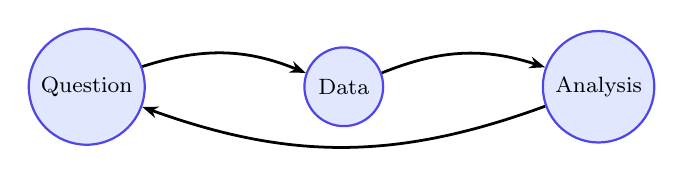
\begin{tikzpicture}[node distance=2cm, auto, thick, every node/.style={font=\footnotesize}]
    \node[circle, draw=customblue, fill=customlightblue, minimum size=1cm] (q) {Question};
    \node[circle, draw=customblue, fill=customlightblue, minimum size=1cm, right=of q] (d) {Data};
    \node[circle, draw=customblue, fill=customlightblue, minimum size=1cm, right=of d] (a) {Analysis};
    
    \draw[-{Stealth[length=2mm]}, line width=1pt] (q) to[bend left=20] (d);
    \draw[-{Stealth[length=2mm]}, line width=1pt] (d) to[bend left=20] (a);
    \draw[-{Stealth[length=2mm]}, line width=1pt] (a) to[bend left=20] (q);
\end{tikzpicture}
\end{center}

\vspace{0.2cm}

\textbf{Embrace iteration}—it's a sign of thorough, careful science
\end{frame}

% Slide 25: Key Takeaways
\begin{frame}{Key Takeaways}

\begin{enumerate}
\item \textbf{Start with clear questions}—they determine everything else

\vspace{0.3cm}
\item \textbf{Good design matters}—randomization, adequate power, controls

\vspace{0.3cm}
\item \textbf{Always visualize first}—avoid Anscombe's Quartet mistakes

\vspace{0.3cm}
\item \textbf{Check assumptions}—models only work when assumptions hold

\vspace{0.3cm}
\item \textbf{Report effect sizes}, not just p-values—statistical $\neq$ biological significance

\vspace{0.3cm}
\item \textbf{Correct for multiple testing}—especially in high-throughput biology

\vspace{0.3cm}
\item \textbf{Communicate clearly}—your science is only as good as your explanation

\vspace{0.3cm}
\item \textbf{Iterate}—real analysis is messy and cyclical
\end{enumerate}
\end{frame}

%%%%%%%%%%%%%%%%%%%%%%%


%\title{Part V: Common Philosophical Tensions in Practice}
%\subtitle{Introduction to Statistics and Data Analysis}
%\author{}
%\date{}

\section{Navigating the fundamental trade-offs in data analysis}
% Slide 1: Title
%\begin{frame}
%\titlepage
%\begin{center}
%\textit{Navigating the fundamental trade-offs in data analysis}
%\end{center}
%\end{frame}

% Slide 2: Overview
\begin{frame}{Three Major Philosophical Tensions}

\textbf{Real data analysis involves navigating fundamental trade-offs:}

\vspace{0.4cm}

\begin{block}{A. Frequentist vs. Bayesian Approaches}
What does probability mean? How should prior knowledge influence analysis?
\end{block}

\begin{block}{B. Prediction vs. Explanation}
Machine learning's predictive power vs. traditional statistics' interpretability
\end{block}

\begin{block}{C. Complexity vs. Simplicity}
The bias-variance tradeoff and Occam's Razor
\end{block}

\vspace{0.4cm}

\begin{center}
\alert{Understanding these tensions makes you a more sophisticated analyst}
\end{center}
\end{frame}

% Slide 3: A - Frequentist vs Bayesian
\begin{frame}{A. Frequentist vs. Bayesian Approaches}
\framesubtitle{Two philosophical frameworks for inference}

\begin{alertblock}{The Core Disagreement}
What does ``probability'' actually mean?
\end{alertblock}

\vspace{0.3cm}

\begin{columns}[T]
\begin{column}{0.48\textwidth}
\begin{block}{Frequentist View}
Probability = \textbf{long-run frequency}

\vspace{0.2cm}
``If we repeated this experiment infinitely many times, what proportion would show this result?''

\vspace{0.2cm}
Parameters are \alert{fixed but unknown}
\end{block}
\end{column}

\begin{column}{0.48\textwidth}
\begin{block}{Bayesian View}
Probability = \textbf{degree of belief}

\vspace{0.2cm}
``Given the evidence, how confident should we be that this is true?''

\vspace{0.2cm}
Parameters are \alert{random variables with distributions}
\end{block}
\end{column}
\end{columns}

\vspace{0.4cm}

\begin{center}
Both are mathematically rigorous—they differ in \alert{philosophy}, not correctness
\end{center}
\end{frame}

% Slide 4: Frequentist Framework
\begin{frame}{The Frequentist Framework}

\textbf{Key concepts:}

\begin{itemize}
\item \textbf{P-values:} Probability of data given null hypothesis
\item \textbf{Confidence intervals:} If we repeated sampling many times, 95\% of CIs would contain true parameter
\item \textbf{Hypothesis testing:} Control long-run error rates ($\alpha$, $\beta$)
\item \textbf{No prior knowledge:} Analysis based only on current data
\end{itemize}

\vspace{0.3cm}

\begin{exampleblock}{Example: Testing Gene Expression}
$H_0$: No difference between treatment and control

\vspace{0.2cm}
Frequentist: ``If there truly is no difference, we'd see data this extreme only 3\% of the time ($p = 0.03$). So we reject $H_0$.''

\vspace{0.2cm}
\alert{Note:} This does NOT tell us probability that $H_0$ is true!
\end{exampleblock}

\vspace{0.3cm}

\textbf{Strengths:} Objective, well-established, controls error rates \\
\textbf{Weaknesses:} Often misinterpreted, can't incorporate prior knowledge
\end{frame}

% Slide 5: Bayesian Framework
\begin{frame}{The Bayesian Framework}

\textbf{Key concepts:}

\begin{itemize}
\item \textbf{Prior distribution:} What we believe before seeing data
\item \textbf{Likelihood:} Probability of data given parameters
\item \textbf{Posterior distribution:} Updated beliefs after seeing data
\item \textbf{Bayes' Theorem:} Posterior $\propto$ Prior $\times$ Likelihood
\end{itemize}

\vspace{0.3cm}

\begin{exampleblock}{Example: Testing Gene Expression}
\textbf{Prior:} Based on literature, most genes don't respond (skeptical prior)

\vspace{0.2cm}
\textbf{Data:} Observe 2-fold change

\vspace{0.2cm}
\textbf{Posterior:} After updating with data, 85\% probability of real effect

\vspace{0.2cm}
Bayesian: ``Given the data and prior knowledge, there's 85\% chance this gene responds to treatment.''
\end{exampleblock}

\vspace{0.3cm}

\textbf{Strengths:} Intuitive interpretation, incorporates prior knowledge \\
\textbf{Weaknesses:} Subjective priors, computationally intensive
\end{frame}

% Slide 6: Example - Rare Disease Testing
\begin{frame}{Example: Rare Disease Testing}
\framesubtitle{When prior knowledge matters}

\begin{exampleblock}{Scenario: Genetic Disease Test}
\textbf{Disease prevalence:} 1 in 10,000 people \\
\textbf{Test accuracy:} 99\% sensitive, 99\% specific \\
\textbf{You test positive.} What's the probability you have the disease?
\pause
\vspace{0.3cm}
\textbf{Intuitive answer:} 99\% (wrong!) \\
\textbf{Correct answer:} Only about 1\%!

\vspace{0.3cm}
\textbf{Why?} In 10,000 people:
\begin{itemize}
\item 1 truly has disease → tests positive (99\% chance)
\item 9,999 don't have disease → 99 test positive (1\% false positive rate)
\item So ~100 positive tests, but only 1 is truly diseased
\item Probability = 1/100 $\approx$ 1\%
\end{itemize}
\end{exampleblock}

\vspace{0.2cm}

\textbf{Lesson:} \alert{Base rates (priors) matter!} Bayesian thinking helps here.
\end{frame}

% Slide 7: When to Use Which
\begin{frame}{Frequentist vs. Bayesian: When to Use Which?}

\begin{block}{Use Frequentist When:}
\begin{itemize}
\item You want to control long-run error rates (clinical trials)
\item No strong prior information exists
\item Regulatory requirements (FDA accepts frequentist)
\item Simple hypothesis testing suffices
\end{itemize}
\end{block}

\begin{block}{Use Bayesian When:}
\begin{itemize}
\item You have strong prior knowledge to incorporate
\item You want direct probability statements about parameters
\item Small sample sizes (priors help stabilize estimates)
\item Complex hierarchical models
\item Sequential updating as data arrives
\end{itemize}
\end{block}

\vspace{0.3cm}

\begin{center}
In biology: \textbf{Frequentist still dominates}, but Bayesian approaches growing \\
\small (especially in genomics, phylogenetics, systems biology)
\end{center}
\end{frame}

% Slide 8: B - Prediction vs Explanation
\begin{frame}{B. Prediction vs. Explanation}
\framesubtitle{Machine learning meets traditional statistics}

\begin{alertblock}{The Tension}
Do we want to \textbf{predict} outcomes accurately or \textbf{understand} the underlying mechanisms?
\end{alertblock}

\vspace{0.3cm}

\begin{columns}[T]
\begin{column}{0.48\textwidth}
\begin{block}{Prediction Focus}
\textbf{Goal:} Maximize accuracy

\vspace{0.2cm}
``Black box'' models OK if they work

\vspace{0.2cm}
\textit{Examples:}
\begin{itemize}
\item Deep neural networks
\item Random forests
\item Gradient boosting
\end{itemize}
\end{block}
\end{column}

\begin{column}{0.48\textwidth}
\begin{block}{Explanation Focus}
\textbf{Goal:} Understand relationships

\vspace{0.2cm}
Interpretability crucial

\vspace{0.2cm}
\textit{Examples:}
\begin{itemize}
\item Linear regression
\item ANOVA
\item Generalized linear models
\end{itemize}
\end{block}
\end{column}
\end{columns}

\vspace{0.4cm}

\begin{center}
Often a \alert{trade-off}: most interpretable models less accurate, \\
most accurate models less interpretable
\end{center}
\end{frame}

% Slide 9: Example - Predicting Disease
\begin{frame}{Example: Predicting Disease Risk}

\begin{exampleblock}{Scenario: Predicting Cancer from Gene Expression}

\textbf{Machine Learning Approach:}
\begin{itemize}
\item Train deep neural network on 10,000 genes
\item Achieves 95\% accuracy on test set
\item But: Can't explain \emph{why} it predicts cancer
\item Can't tell which genes matter most
\end{itemize}

\vspace{0.3cm}

\textbf{Statistical Modeling Approach:}
\begin{itemize}
\item Logistic regression with 5 key genes (from prior knowledge)
\item Achieves 88\% accuracy
\item Can interpret: Each unit increase in Gene A multiplies odds by 2.5
\item Can validate biological mechanism
\end{itemize}
\end{exampleblock}

\vspace{0.3cm}

\textbf{Which is better?} \alert{Depends on your goal!}
\end{frame}

% Slide 10: When Prediction Matters
\begin{frame}{When to Prioritize Prediction}

\textbf{Prediction is the primary goal when:}

\vspace{0.3cm}

\begin{itemize}
\item \textbf{Clinical decision support} — Need accurate diagnosis/prognosis \\
\small \textit{Example:} Predicting patient response to immunotherapy

\vspace{0.2cm}
\item \textbf{Screening/classification} — Identify candidates for further study \\
\small \textit{Example:} Identifying potential drug compounds from chemical structure

\vspace{0.2cm}
\item \textbf{Mechanism partially known} — Just need to predict outcome \\
\small \textit{Example:} Predicting protein structure from sequence (we know physics, but it's complex)

\vspace{0.2cm}
\item \textbf{Validation available} — Can test predictions experimentally \\
\small \textit{Example:} ML predicts gene function → validate with knockout
\end{itemize}

\vspace{0.3cm}

\begin{center}
If the model works and improves decisions, \alert{interpretability is secondary}
\end{center}
\end{frame}

% Slide 11: When Explanation Matters
\begin{frame}{When to Prioritize Explanation}

\textbf{Explanation is the primary goal when:}

\vspace{0.3cm}

\begin{itemize}
\item \textbf{Basic science} — Want to understand biological mechanisms \\
\small \textit{Example:} Which genes regulate cell cycle progression?

\vspace{0.2cm}
\item \textbf{Hypothesis generation} — Need to guide future experiments \\
\small \textit{Example:} What pathways are perturbed in disease?

\vspace{0.2cm}
\item \textbf{Intervention design} — Need to know what to manipulate \\
\small \textit{Example:} Which metabolic enzyme to target with drug?

\vspace{0.2cm}
\item \textbf{Trust and transparency} — Stakeholders need to understand \\
\small \textit{Example:} Explaining treatment decisions to patients

\vspace{0.2cm}
\item \textbf{Scientific publishing} — Reviewers expect mechanistic insight \\
\small \textit{Example:} Most biological journals want causal stories
\end{itemize}

\vspace{0.3cm}

\begin{center}
If you can't explain it, you don't really \alert{understand} it
\end{center}
\end{frame}

% Slide 12: Middle Ground
\begin{frame}{Finding the Middle Ground}

\textbf{Strategies to balance prediction and explanation:}

\vspace{0.3cm}

\begin{enumerate}
\item \textbf{Interpretable ML models} \\
\small Use methods like LASSO, elastic net, decision trees that offer some interpretability

\vspace{0.2cm}
\item \textbf{Post-hoc interpretation} \\
\small Apply SHAP values, feature importance, or partial dependence plots to black boxes

\vspace{0.2cm}
\item \textbf{Two-stage approach} \\
\small Use ML for prediction, then simpler models to understand top features

\vspace{0.2cm}
\item \textbf{Mechanistic ML} \\
\small Incorporate biological constraints into neural networks

\vspace{0.2cm}
\item \textbf{Ensemble thinking} \\
\small Use both approaches and compare insights
\end{enumerate}

\vspace{0.3cm}

\begin{alertblock}{}
\centering
The best approach depends on your \alert{scientific question} and \alert{available data}
\end{alertblock}
\end{frame}

% Slide 13: C - Complexity vs Simplicity
\begin{frame}{C. Complexity vs. Simplicity}
\framesubtitle{The bias-variance tradeoff}

\begin{block}{The Fundamental Tradeoff}
\begin{itemize}
\item \textbf{Simple models:} May miss important patterns (high bias)
\item \textbf{Complex models:} May fit noise as if it were signal (high variance)
\end{itemize}
\end{block}

\vspace{0.3cm}

\begin{center}
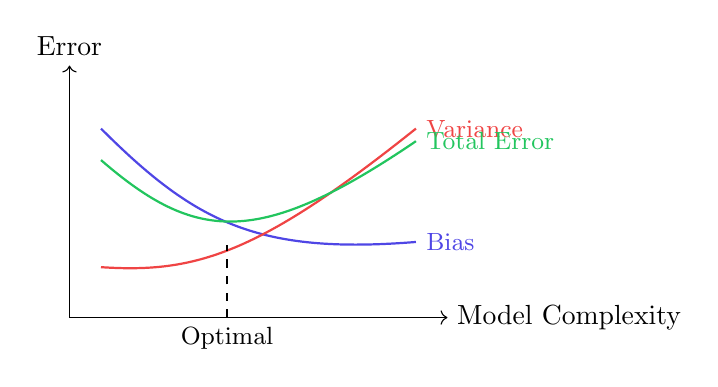
\begin{tikzpicture}[scale=0.8]
    % Axes
    \draw[->] (0,0) -- (6,0) node[right] {Model Complexity};
    \draw[->] (0,0) -- (0,4) node[above] {Error};
    
    % Curves
    \draw[thick, customblue] (0.5,3) .. controls (2,1.5) and (3,1) .. (5.5,1.2) node[right] {\small Bias};
    \draw[thick, customred] (0.5,0.8) .. controls (2,0.7) and (3,1) .. (5.5,3) node[right] {\small Variance};
    \draw[thick, customgreen] (0.5,2.5) .. controls (2,1.2) and (3,1.1) .. (5.5,2.8) node[right] {\small Total Error};
    
    % Optimal point
    \draw[dashed] (2.5,0) -- (2.5,1.15);
    \node[below] at (2.5,0) {\small Optimal};
\end{tikzpicture}
\end{center}

\vspace{0.2cm}

\textbf{Goal:} Find the sweet spot that minimizes \alert{total error}
\end{frame}

% Slide 14: Underfitting vs Overfitting
\begin{frame}{Underfitting vs. Overfitting}

\begin{columns}[T]
\begin{column}{0.32\textwidth}
\begin{block}{Underfitting}
\small
\textbf{Problem:} Model too simple

\vspace{0.2cm}
\textbf{Symptoms:}
\begin{itemize}
\item Poor fit to data
\item High error on training set
\item High error on test set
\end{itemize}

\vspace{0.2cm}
\textbf{Example:} Linear model for curved relationship
\end{block}
\end{column}

\begin{column}{0.32\textwidth}
\begin{block}{Just Right}
\small
\textbf{Balance:} Captures signal, ignores noise

\vspace{0.2cm}
\textbf{Symptoms:}
\begin{itemize}
\item Good fit to data
\item Low training error
\item Low test error
\end{itemize}

\vspace{0.2cm}
\textbf{Example:} Polynomial degree matches true curve
\end{block}
\end{column}

\begin{column}{0.32\textwidth}
\begin{block}{Overfitting}
\small
\textbf{Problem:} Model too complex

\vspace{0.2cm}
\textbf{Symptoms:}
\begin{itemize}
\item Perfect fit to data
\item Very low training error
\item High test error
\end{itemize}

\vspace{0.2cm}
\textbf{Example:} High-degree polynomial fits noise
\end{block}
\end{column}
\end{columns}

\vspace{0.4cm}

\begin{alertblock}{}
\centering
\alert{Training error always decreases} with complexity, but \alert{test error may increase!}
\end{alertblock}
\end{frame}

% Slide 15: Example - Growth Curves
\begin{frame}{Example: Modeling Bacterial Growth}

\begin{exampleblock}{Scenario: Fitting Growth Curve to 10 Time Points}

\textbf{Model 1: Linear} (too simple)
\begin{itemize}
\item Misses exponential phase
\item High error
\item Underfits
\end{itemize}

\vspace{0.2cm}

\textbf{Model 2: Logistic curve} (just right)
\begin{itemize}
\item Captures lag, exponential, stationary phases
\item Biologically motivated
\item Generalizes well
\end{itemize}

\vspace{0.2cm}

\textbf{Model 3: 9th-degree polynomial} (too complex)
\begin{itemize}
\item Passes through every point perfectly
\item Wiggles unrealistically between points
\item Terrible predictions for new data
\item Overfits
\end{itemize}
\end{exampleblock}
\end{frame}

% Slide 16: Occam's Razor
\begin{frame}{Occam's Razor in Statistics}

\begin{block}{Principle of Parsimony}
\textit{``Among competing hypotheses that explain the data equally well, \\
the simplest one is most likely to be correct''}
\end{block}

\vspace{0.3cm}

\textbf{Why prefer simpler models?}

\begin{itemize}
\item \textbf{Interpretability} — Easier to understand and communicate
\item \textbf{Generalizability} — Less likely to overfit
\item \textbf{Stability} — Small data changes don't drastically alter model
\item \textbf{Falsifiability} — Simpler hypotheses easier to test
\item \textbf{Biological plausibility} — Nature often operates by simple principles
\end{itemize}

\vspace{0.3cm}

\begin{alertblock}{}
\centering
\alert{But:} Don't oversimplify! Use as complex a model as needed, but no more
\end{alertblock}
\end{frame}

% Slide 17: Tools for Model Selection
\begin{frame}{Tools for Balancing Complexity}

\textbf{How to choose model complexity:}

\vspace{0.3cm}

\begin{block}{Cross-Validation}
Split data into training/test sets; evaluate performance on held-out data \\
\small Most reliable method for assessing generalization
\end{block}

\begin{block}{Information Criteria}
\textbf{AIC} (Akaike) / \textbf{BIC} (Bayesian): Balance fit and complexity \\
\small Lower values = better; BIC penalizes complexity more heavily
\end{block}

\begin{block}{Regularization}
Add penalty for model complexity (LASSO, Ridge, Elastic Net) \\
\small Automatically shrinks unimportant coefficients toward zero
\end{block}

\vspace{0.3cm}

\begin{exampleblock}{Example in RNA-seq}
You have 20,000 genes but only 50 samples → severe overfitting risk \\
Solution: Use LASSO to select most important genes automatically
\end{exampleblock}
\end{frame}

% Slide 18: Example - Predictive Modeling
\begin{frame}{Example: Predicting Protein Expression}

\begin{exampleblock}{Scenario: Predict protein levels from mRNA}

\textbf{Available predictors:}
\begin{itemize}
\item mRNA abundance (obvious choice)
\item mRNA half-life
\item Codon usage
\item 5' UTR structure
\item Ribosome binding site strength
\item ... 50 other features
\end{itemize}

\vspace{0.3cm}

\textbf{Approach 1:} Include all 50+ features \\
\textbf{Problem:} Perfect fit to training data, terrible predictions (overfitting)

\vspace{0.3cm}

\textbf{Approach 2:} Use only mRNA abundance \\
\textbf{Problem:} Misses important biology (underfitting)

\vspace{0.3cm}

\textbf{Approach 3:} Use LASSO or cross-validation to select 5-10 key features \\
\textbf{Result:} Good predictions, interpretable, captures main biology
\end{exampleblock}
\end{frame}

% Slide 19: Domain Knowledge
\begin{frame}{The Role of Domain Knowledge}

\begin{alertblock}{Key Insight}
In biology, \alert{domain knowledge} should guide the bias-variance tradeoff
\end{alertblock}

\vspace{0.3cm}

\textbf{Use biological knowledge to:}

\begin{itemize}
\item \textbf{Choose functional forms} \\
\small Use mechanistic equations (Michaelis-Menten, Hill, logistic) rather than arbitrary polynomials

\vspace{0.2cm}
\item \textbf{Select variables} \\
\small Include biologically relevant predictors, exclude implausible ones

\vspace{0.2cm}
\item \textbf{Set constraints} \\
\small Force parameters to be positive, bounded, etc. based on biology

\vspace{0.2cm}
\item \textbf{Interpret results} \\
\small If model suggests implausible biology, probably overfitting
\end{itemize}

\vspace{0.3cm}

\begin{center}
\textbf{Don't let the algorithm alone decide}—inject biological reasoning!
\end{center}
\end{frame}

% Slide 20: When to Accept Complexity
\begin{frame}{When Complex Models Are Justified}

\textbf{Sometimes complexity is necessary:}

\vspace{0.3cm}

\begin{itemize}
\item \textbf{Biological systems are complex} \\
\small Gene networks, metabolic pathways, ecosystems—reality has many interactions

\vspace{0.2cm}
\item \textbf{Large datasets support it} \\
\small With millions of data points (genomics), can fit complex models reliably

\vspace{0.2cm}
\item \textbf{Prediction is the goal} \\
\small If you just need accurate forecasts, complexity OK if validated

\vspace{0.2cm}
\item \textbf{Simple models demonstrably fail} \\
\small If linear model gives terrible fit and residuals show clear patterns
\end{itemize}

\vspace{0.3cm}

\begin{alertblock}{}
\centering
The principle is not \alert{``always use simple models''} but \\
\alert{``use the simplest model that adequately captures the biology''}
\end{alertblock}
\end{frame}

% Slide 21: Navigating All Three Tensions
\begin{frame}{Navigating All Three Tensions Together}

\textbf{Real analysis involves all three tensions simultaneously:}

\vspace{0.3cm}

\begin{exampleblock}{Example: Analyzing Clinical Trial Data}

\textbf{Frequentist vs. Bayesian:}
\begin{itemize}
\item Should we incorporate prior trial results? (Bayesian)
\item Or analyze this trial independently? (Frequentist)
\end{itemize}

\textbf{Prediction vs. Explanation:}
\begin{itemize}
\item Do we need to predict individual response? (ML)
\item Or understand which factors matter? (Statistical modeling)
\end{itemize}

\textbf{Complexity vs. Simplicity:}
\begin{itemize}
\item Include all patient characteristics? (Complex)
\item Or just treatment group? (Simple)
\end{itemize}

\vspace{0.2cm}

\textbf{Decision depends on:} Study goals, sample size, regulatory requirements, stakeholder needs
\end{exampleblock}
\end{frame}

% Slide 22: Practical Guidance
\begin{frame}{Practical Guidance for Biological Research}

\textbf{General recommendations:}

\vspace{0.3cm}

\begin{enumerate}
\item \textbf{Start simple, add complexity only if needed} \\
\small Fit basic model first; add terms only if significantly improve fit

\vspace{0.2cm}
\item \textbf{Use biological knowledge to constrain choices} \\
\small Don't treat analysis as pure math—inject domain expertise

\vspace{0.2cm}
\item \textbf{Validate, validate, validate} \\
\small Use held-out data, cross-validation, independent replication

\vspace{0.2cm}
\item \textbf{Match method to question} \\
\small Prediction task? ML is fine. Causal inference? Need careful design

\vspace{0.2cm}
\item \textbf{Be transparent about choices} \\
\small Report why you chose Bayesian vs. frequentist, complex vs. simple

\vspace{0.2cm}
\item \textbf{Consider multiple approaches} \\
\small Try both frequentist and Bayesian; compare simple and complex models
\end{enumerate}
\end{frame}

% Slide 23: No Perfect Answer
\begin{frame}{There Is No Perfect Answer}

\begin{center}
\Large \alert{All of these tensions involve genuine trade-offs} \\
\vspace{0.3cm}
\large There is no universally ``correct'' choice
\end{center}

\vspace{0.4cm}

\textbf{What matters is:}

\begin{itemize}
\item \textbf{Awareness} — Recognize these tensions exist
\item \textbf{Thoughtfulness} — Make deliberate choices based on context
\item \textbf{Transparency} — Explain and justify your decisions
\item \textbf{Humility} — Acknowledge limitations of your approach
\item \textbf{Iteration} — Be willing to try alternative approaches
\end{itemize}

\vspace{0.4cm}

\begin{block}{}
\centering
\textbf{The mark of a sophisticated analyst:} \\
Understanding the trade-offs and navigating them wisely
\end{block}
\end{frame}

% Slide 24: Key Takeaways
\begin{frame}{Key Takeaways}

\begin{enumerate}
\item \textbf{Frequentist vs. Bayesian:} Different philosophies of probability; choose based on goals and whether prior knowledge exists

\vspace{0.3cm}
\item \textbf{Prediction vs. Explanation:} ML excels at prediction; statistical models provide understanding. Match method to question

\vspace{0.3cm}
\item \textbf{Complexity vs. Simplicity:} Balance bias and variance. Use cross-validation and information criteria to find sweet spot

\vspace{0.3cm}
\item \textbf{Occam's Razor:} Prefer simpler models when they explain data equally well, but don't oversimplify complex biology

\vspace{0.3cm}
\item \textbf{Domain knowledge:} Use biological understanding to guide statistical choices

\vspace{0.3cm}
\item \textbf{No perfect answer:} These are genuine trade-offs; thoughtful navigation matters more than finding the ``right'' approach
\end{enumerate}
\end{frame}

% Slide 25: Conclusion
\begin{frame}{Conclusion: Becoming a Thoughtful Analyst}

\begin{center}
\Large Understanding these philosophical tensions \\
\vspace{0.2cm}
transforms you from a \alert{button-pusher} \\
\vspace{0.2cm}
into a \alert{thoughtful scientist}
\end{center}

\vspace{0.5cm}

\textbf{Key principles for practice:}

\begin{itemize}
\item Question your assumptions
\item Understand your tools deeply
\item Match methods to questions
\item Validate rigorously
\item Communicate transparently
\item Stay humble about uncertainty
\end{itemize}

\vspace{0.4cm}

\begin{center}
\colorbox{myOrange}{\textcolor{white}{\parbox{0.9\textwidth}{\centering\textbf{Good data analysis is both a science and an art—\\master the philosophy as well as the techniques}}}}
\end{center}
\end{frame}

\begin{frame}{Syllabus}
	\begin{itemize}
		\item Introduction
		\item Probability and descriptive statistics
		\item Statistical Inference
		\item Linear Models
		\item Basics of Experimental Design
	\end{itemize}

\end{frame}

\end{document}
